\documentclass[11pt]{article}
\usepackage[english]{babel}
\usepackage[latin1]{inputenc}
\usepackage{lmodern}
\usepackage[T1]{fontenc}
\usepackage[outer=3.75cm, marginparwidth=4.5cm]{geometry}
%\usepackage{marginnote}
\usepackage{amssymb,amsmath,amsthm,latexsym,amsfonts,amscd,dsfont,enumerate,bbm,mathabx}
\usepackage{graphicx,tikz}
\usepackage{draftwatermark}
\usepackage{enumerate} 
% \usepackage{listings}
% \usepackage{booktabs}
\usepackage{mathtools}
% \usepackage[gen]{eurosym}
% \usepackage{algorithm}
% \usepackage{algpseudocode}
\usepackage{soul}
\usepackage{comment}
\usepackage{bm}
\usepackage[font=small,labelfont=bf]{caption}
\graphicspath{{Local_Volatility/}{Black_Scholes/}}
% \setbeamertemplate{bibliography item}[text]
% \renewcommand*{\bibfont}{\scriptsize}

% \usepackage{pgfplots}
% \pgfplotsset{compat=newest}

\definecolor{mylightyellow}{rgb}{1,1,.8}
\definecolor{mylightgreen}{rgb}{.8,1,.8}
\definecolor{mydarkred}{RGB}{178,34,34}
\definecolor{mydarkgreen}{RGB}{34,139,34}
\definecolor{mydarkblue}{RGB}{72,61,139}
\definecolor{mydarkyellow}{RGB}{218,165,32}

\definecolor{myblueA}{RGB}{52,41,39}
\definecolor{myblueB}{RGB}{92,81,109}
\definecolor{myblueC}{RGB}{132,121,179}
\definecolor{myblueD}{RGB}{172,161,249}
\definecolor{myblueE}{RGB}{212,201,255}

\usetikzlibrary{arrows,patterns,shapes,snakes,shadows,fit,backgrounds,positioning,decorations.pathmorphing,external}
\tikzstyle{nameusd} = [circle, draw, top color=white, bottom color=mydarkblue!50, draw=mydarkblue!75!black!100, drop shadow, minimum height=4em]
\tikzstyle{nameeur} = [circle, draw, top color=white, bottom color=mydarkred!50, draw=mydarkred!75!black!100, drop shadow, minimum height=4em]
\tikzstyle{collusd} = [rectangle,fill=mydarkblue!10, inner sep=0.2cm, rounded corners=5mm]
\tikzstyle{colleur} = [rectangle,fill=mydarkred!10, inner sep=0.2cm, rounded corners=5mm]
\tikzstyle{fixto} = [draw, -latex']
\tikzstyle{fixfrom} = [draw, latex'-]
\tikzstyle{floatto} = [draw, snake=coil, segment aspect=0, line before snake=2ex, line after snake=1ex, -latex']
\tikzstyle{floatfrom} = [draw, snake=coil, segment aspect=0, line before snake=2ex, line after snake=1ex, latex'-]
\tikzstyle{investor} = [rectangle, draw, top color=white, bottom color=mydarkyellow!50, draw=mydarkyellow!75!black!100, drop shadow, rounded corners, minimum height=3em, text width=4em, text centered]
\tikzstyle{trader} = [circle, draw, top color=white, bottom color=blue!30, draw=blue!50!black!100, drop shadow, minimum height=4em]
\tikzstyle{bank} = [rectangle, draw, top color=white, bottom color=red!20, draw=red!50!black!100, drop shadow, rounded corners, minimum height=3em, text width=4em, text centered]
\tikzstyle{market} = [rectangle, draw, top color=white, bottom color=green!20, draw=green!50!black!100, drop shadow, rounded corners, minimum height=3em, text width=4em, text centered]
\tikzstyle{yellowbox} = [rectangle, draw, top color=white, bottom color=mydarkyellow!50, draw=mydarkyellow!75!black!100, drop shadow, rounded corners, text centered]
\tikzstyle{fadedyellowbox} = [rectangle, draw=gray, text=gray, top color=white, bottom color=mydarkyellow!25, draw=mydarkyellow!50, drop shadow, rounded corners, text centered]
\tikzstyle{redbox} = [rectangle, draw, top color=white, bottom color=mydarkred!50, draw=mydarkred!75!black!100, drop shadow, rounded corners, text centered]
\tikzstyle{fadedredbox} = [rectangle, draw=gray, text=gray, top color=white, bottom color=mydarkred!25, draw=mydarkred!50, drop shadow, rounded corners, text centered]
\tikzstyle{bluebox} = [rectangle, draw, top color=white, bottom color=mydarkblue!50, draw=mydarkblue!75!black!100, drop shadow, rounded corners, text centered]
\tikzstyle{fadedbluebox} = [rectangle, draw=gray, text=gray, top color=white, bottom color=mydarkblue!25, draw=mydarkblue!50, drop shadow, rounded corners, text centered]
\tikzstyle{greenbox} = [rectangle, draw, top color=white, bottom color=mydarkgreen!50, draw=mydarkgreen!75!black!100, drop shadow, rounded corners, text centered]
\tikzstyle{fadedgreenbox} = [rectangle, draw=gray, text=gray, top color=white, bottom color=mydarkgreen!25, draw=mydarkgreen!50, drop shadow, rounded corners, text centered]

\newcommand{\tikzmark}[1]{\tikz[remember picture] \node[coordinate] (#1) {#1};}

% \pgfplotstableread{data/total_consumption_example.dat}\swingtotal

\usepackage[]{hyperref}
\hypersetup{
	colorlinks=true,breaklinks=true,
	urlcolor= mydarkblue,linkcolor= mydarkblue,citecolor= mydarkgreen,
	pdfauthor={Daluiso, R., Nastasi, E., Pallavicini, A., Polo, S.},
}
\usepackage[backend=biber,style=authoryear-comp,maxcitenames=2,sorting=nyt,natbib=true,sortcites=false]{biblatex}
\setlength\bibitemsep{1.3\itemsep}

\addbibresource{Bib.bib}
%\usepackage{natbib}
%\setcitestyle{authoryear,open={(},close={)}}
\newtheorem{theorem}{Theorem}[section]
\newtheorem{lemma}[theorem]{Lemma}
\newtheorem{proposition}[theorem]{Proposition}
\newtheorem{corollary}{Corollary}[theorem]
\newtheorem{remark}{Remark}[section]
\newtheorem{example}[remark]{Example}

\newcommand{\Eq}[1]{{\begin{equation}{#1}\end{equation}}}

\newcommand{\Exo}[1]{\mathbb{E}\!\left[\,#1\,\right]}
\newcommand{\Ex}[2]{\mathbb{E}_{#1}\!\left[\,#2\,\right]}
\newcommand{\ExG}[2]{\mathbb{E}\!\left[\,#2\,\left|{\cal G}_{#1}\right.\right]}
\newcommand{\ExF}[2]{\mathbb{E}\!\left[\,#2\,\left|{\cal F}_{#1}\right.\right]}
\newcommand{\ExFT}[3]{\mathbb{E}^{#2}\!\left[\,#3\,\left.\right|{\cal F}_{#1}\right]}
\newcommand{\ExGT}[3]{\mathbb{E}^{#2}\!\left[\,#3\,\left.\right|{\cal G}_{#1}\right]}
\newcommand{\ExCo}[2]{\mathbb{E}\!\left[\left.\,#1\,\right|\,#2\,\right]}
\newcommand{\ExC}[3]{\mathbb{E}_{#1}\!\left[\left.\,#2\,\right|\,#3\,\right]}
\newcommand{\ExCT}[4]{\mathbb{E}_{#1}^{#2}\!\left[\left.\,#3\,\right|\,#4\,\right]}
\newcommand{\ExT}[3]{\mathbb{E}_{#1}^{#2}\!\left[\,#3\,\right]}
\newcommand{\Exf}[2]{\hat{\mathbb{E}}_{#1}\!\left[\,#2\,\right]}
\newcommand{\ExfT}[3]{\hat{\mathbb{E}}_{#1}^{#2}\!\left[\,#3\,\right]}
\newcommand{\Px}[1]{\mathbb{P}\left\{\,#1\,\right\}}
\newcommand{\PxC}[2]{\mathbb{P}\!\left\{\,#1\,\left.\right|\,#2\,\right\}}
\newcommand{\Qx}[1]{\mathbb{Q}\left\{\,#1\,\right\}}
\newcommand{\QxC}[2]{\mathbb{Q}\!\left\{\,#1\,\left.\right|\,#2\,\right\}}
\newcommand{\QxCT}[3]{\mathbb{Q}^{#1}\!\left\{\,#2\,\left.\right|\,#3\,\right\}}
\newcommand{\QxT}[2]{\mathbb{Q}^{#1}\left\{\,#2\,\right\}}
\newcommand{\Qxf}[1]{\hat{\mathbb{Q}}\left\{\,#1\,\right\}}
\newcommand{\Var}[2]{\operatorname{Var}_{#1}\!\left[\,#2\,\right]}
\newcommand{\Covar}[3]{\operatorname{Covar}_{#1}\!\left[\,#2,#3\,\right]}
\newcommand{\ind}[1]{1_{\{#1\}}}
\newcommand{\clip}[3]{\operatorname{clip}\!\left({#1},{#2},{#3}\right)}
\newcommand{\one}{\ensuremath{\mathbbm{1}}}
\newcommand{\onehalf}{\tfrac{1}{2}}

\newcommand{\tr}[1]{{#1}^{\intercal}} %transpose
\DeclareMathOperator{\Tr}{Tr}
\let\oldnorm\norm   % <-- Store original \norm as \oldnorm
\let\norm\undefined % <-- "Undefine" \norm
\DeclarePairedDelimiter\norm{\lVert}{\rVert}

\newcommand{\rec}{R}
\newcommand{\lgd}{\mbox{L{\tiny GD}}}
\newcommand{\virgolette}[1]{``#1''}
\newcommand{\pvcall}{{\mathcal{C}}}
\newcommand{\pvput}{{\mathcal{P}}}

\usepackage{eurosym}
\newcommand{\euroms}[0]{\mbox{\small \euro}}
\usepackage{cleveref}
\DeclareMathOperator*{\argmax}{arg\,max}
\DeclareMathOperator*{\argmin}{arg\,min}

\newenvironment{eqsys}{\begin{equation}\begin{dcases}}{\end{dcases}\end{equation}}
\usepackage{fancyhdr}
\renewcommand{\headrulewidth}{0pt}
\fancyhead[R]{}
\lhead{\footnotesize\slshape Daluiso, Nastasi, Pallavicini, Polo, Optimal Strategies for Target Volatility Contracts}
\chead{}
\rhead{\thepage}
\lfoot{}
\cfoot{}
\rfoot{}

%%%%%%%%%%%%%%%%%%%%%%%%%%%%%%%%%%%%%%%%%%%%%%%%%%%%%%%%%%%%%%%%%%%%%


\title{Reinforcement Learning for Options on Target Volatility Funds}

\author{
	Roberto Daluiso\thanks{Intesa Sanpaolo Milan, roberto.daluiso@intesasanpaolo.com}
	\and 
	Emanuele Nastasi\thanks{Marketz S.p.A., emanuele.nastasi@marketz.eu}
	\and Andrea Pallavicini\thanks{Imperial College London and Intesa Sanpaolo Milan, a.pallavicini@imperial.ac.uk} 
	\and
	Stefano Polo\thanks{Intesa Sanpaolo Milan, stefano.polo@intesasanpaolo.com} 
}

%\date{
%	First Version: March 2021. This Version: \today
%}
\begin{document} % goes here

\maketitle

\begin{abstract}
\noindent In recent years Reinforcement Learning (RL) techniques are gaining popularity in the field of quantitative finance since they are proving to be an efficient way to solve  high-dimensional optimal control problems. 
Our research project is devoted to apply RL to price derivative contracts on target volatility strategies (TVSs), portfolios of risky assets and a risk-free one dynamically rebalanced in order to keep the realized volatility of the portfolio on a certain level. The uncertainty in the TVS risky portfolio composition along with the difference in hedging costs for each component requires to solve a stochastic control problem to evaluate the option prices. The topic of hedging costs is a novelty never dealt in the TVS literature and we provide a formal description of the entire control problem. We tackle the problem by implementing a RL algorithm to determine the optimal risky portfolio composition leading to the most conservative option price.  We investigate the problem for two models of the risky asset dynamics: time-dependent Black and Scholes and local volatility. In the first case we prove the existence of an analytical solution of the problem; a result that we use as benchmark to perform a series of fine-tuning of the RL hyper-parameters. At the end we provide numerical results for the local volatility model, for which an \textit{a priori} solution is not available.
\end{abstract}

\smallskip
\noindent
\textbf{JEL classification codes:} C63, C45, C61, G11, G13.\\
\textbf{AMS classification codes:} 65C05, 91G20, 91G60.\\
\textbf{Keywords:} Reinforcement Learning, Hedging Costs, Funding Costs, Proximal Policy Optimization, Target Volatility, Asset Allocation. 
\newpage
\tableofcontents
 \mbox{}
 \vfill
 \noindent \small The opinions here expressed are solely those of the authors and do not represent in any way those of their employers.

\newpage
\pagestyle{myheadings} \markboth{}{{\footnotesize Daluiso, Pallavicini, Nastasi, Polo, Reinforcement Learning for Options on Target Volatility Funds}}
\section{Introduction}
In the recent years portfolio managers are exposed to very low interest rates and quickly changing market volatilities. An effective solution to control risks under such environment is given by target volatility strategies (TVSs) (also known as constant volatility targeting) which are able to preserve the portfolio at a predetermined level of volatility. A TVS is  a  portfolio  of  risky  assets  (typically  equities)  and  a  risk-free  asset dynamically re-balanced with the aim of maintaining the overall portfolio volatility level closed to some target value. This products were initially offered in the Asian markets, see for instance the reports of \textcite{Chew} and \textcite{XUE} which highlight the pros and cons for investors, to be adopted in the following years in many other markets in North America and Europe as depicted in \textcite{Morrison}.

In literature TVSs are tested to investigate their performances in term of realized returns, see for instance \textcite{Hocquard28} and \textcite{PERCHET}, and the soundness of the volatility targeting algorithm, as described in \textcite{Kim}. Moreover, in pricing literature, derivative contracts on TVS, known as target volatility options (TVOs), are studied, see in particular \textcite{Di_Graziano}, \textcite{Grasselli}, and \textcite{Albeverio}. 

In this contribution we face a new topic never dealt with in the TVS literature: the funding costs coming from hedging the risky assets underlying the TVS. We consider the point of view of a bank selling a call option to a portfolio manager as protection on the capital invested in a TVS. The portfolio manager has the freedom of changing the relative weights of the risky assets during the life of the TVS. Since the risky assets have different hedging costs, the bank shall adjust the price of the protection to include them in the worst-case scenario, i.e. the most expensive strategy from the financing costs point of view. Hence, the pricing problem becomes a dynamical control problem over the risky portfolio composition. In our contribution we describe the dynamical control problem, and we derive an analytical solution in the simple case of the risky assets driven by a Black-Scholes (BS) model \citep{BlackScholes}. Then, we tackle the problem in the general case of a local volatility (LV) model \citep{Dupire94pricingwith,LVfirst} by using Reinforcement Learning (RL) algorithms, in particular the proximal policy optimization developed in \textcite{ppo}.
\\

The paper is organized ad follows. In \Cref{sec:TVS} we describe the dynamics of a TVS in presence of valuation adjustments. Then, in \Cref{sec:Derivative} we study the case of derivative contracts on TVSs, we describe the dynamical control problem giving the expression of the Hamilton-Jacobi-Bellman equation and we derive the analytical results for plain vanilla options under BS dynamics. In \Cref{sec:RL} we illustrate how we have applied RL to solve the dynamic control problem, giving a description of the algorithm we have built. We conclude the paper with \Cref{sec:Numerical_results} where we present the numerical results obtained in this work for the Black and Scholes model and the local volatility one.
\\

A part of this work has been developed during the Master thesis of one of us (SP), where we had the opportunity to collaborate with Marco Bianchetti and Diego Pierluigi Giovannini from Intesa Sanpaolo, Milan, that we tanks. Moreover we wish to thank the Italian computing centre Cineca, which approved our ISCRA C project and provided us the high-computing resources of Marconi100 for the numerical simulations of this contribution.


\section{Target Volatility Strategy}\label{sec:TVS}
In a TVS the fund manager selects an allocation strategy aiming at stabilizing the portfolio volatility to a target level. Clients investing in the fund pay a running fee for the service and their capital is protected. The fund manager usually buys an option on the TVS to ensure capital protection. For instance, the capital can be protected by buying a put option. In this case, we can write the net asset value (NAV) $A_t$ of the strategy as given by\footnote{Here we neglect discounting factors.}
\begin{equation}
    A_t \coloneqq \max\{V_t,K\} = V_t + (K-V_t)^+,
\end{equation}
where $V_t$ is the price process of the strategy, and $K$ is the guaranteed capital. On the other hand, the fund manager can replicate the payoff by means of the put-call parity by investing the capital in a low-risk asset and buying a call on the strategy
\begin{equation}
    A_t = K + (V_t-K)^+.
\end{equation}
In this way the TVS is only defined in the two contracts client-fund and fund-bank. The fund manager is not implementing the strategy by trading in the market, and he is not subject to additional costs to access the market. On the other way, the bank is paying such costs since she is actively hedging the call option sold to the manager. 

The bank trading activity implemented to actively hedge the option requires funding the collateral procedures of the hedging instruments along with any lending/borrowing fee. The price of a financial product sold by the bank is modified to include any valuation adjustment due to the trading activity. We proceed by defining the price process for the TVS so that we can highlights the impact of valuation adjustments.
\subsection{The strategy Price Process}
We work on a filtered probability space $\left(\Omega, \mathcal{F}, \{\mathcal{F}_t\}_{t\geq0}, \mathbb{P}  \right)$ satisfying the usual assumptions for a market model, where $\mathbb{P}$ is the physical probability measure representing the actual distribution of supply and demand shocks on equities prices. 

We consider a fund trading a basket of $n$ risky securities with price process $S_t^i$ with $i=1,\dots,n$ funded with a cash account $B_t$ accruing at $r_t$. Any dividend paid by the securities is re-invested in the fund, so that we limit our analysis to total return securities, namely we assume that holding the security is self-financing. Here, we assume that the TVS is implemented in continuous time, even if in the practice we can implement the strategy only on a discrete set of dates. We introduce the deflated gain process $\Bar{G}_t^i$ associated to the risky securities as given by
\begin{equation}
    \Bar{G}_t^i \coloneqq \Bar{S}_t^i + \Bar{D}_t^i,
\end{equation}
where we define the deflated price\footnote{We use bar notation for deflated quantities: processes expressed in terms of $B_t$.} and cumulative dividend processes as 
\begin{equation}
    \bar{S}_t^i \coloneqq \frac{S_t^i}{B_t}, \quad \bar{D}^i_t \coloneqq \int_0^t\frac{d\pi_u^i}{B_u} + \int_0^t\frac{d\psi_u^i}{B_u},
\end{equation}
where $\pi^i_t$ represents the cumulative contractual-coupon process paid by the security, and $\psi_t^i$ represents the cumulative valuation adjustments.

Valuation adjustments (XVAs) is a topic widely discussed in the literature. We refer to \textcite{Brigo} for a discussion. Since fund managers allocating TVS usually rely on Equity assets, here we use the results of \textcite{Gabrielli} which  analyze the valuation adjustments for equity products. We can write
\begin{equation}
    \psi_t^i \coloneqq \int_0^t S_u^i\mu_u^i du,
\label{eq:XVA_equity}\end{equation}
where we call $\mu_t^i$ cost of carry, which basically represents the hedging costs for the $i$-th security.

Then, we introduce the strategy price process $V_t$, and we define the deflated gain process $\Bar{G}_t^V$ as given by
\begin{equation}
    \Bar{G}_t^V \coloneqq \frac{V_t}{B_t} + \int_0^t\frac{V_u\phi_u}{B_u}du,
\end{equation}
where $\phi_t$ are the running fees earned by the fund manager for his activity. We assume that the strategy is self-financing, so that we can write
\begin{equation}
    d\Bar{G}_t^V = q_t \cdot d\bar{G}_t,
\label{eq:self_financing}\end{equation}
where $q_t^i$ is the quantity invested in the $i$-th security\footnote{In all formulae we use dot notation for scalar product between vectors, i.e. $a \cdot b = \sum_i a_i b_i$, or between matrix and vector, i.e. $A \cdot b = \sum_j a_{ij}b_j$ or $b \cdot A = \sum_i b_i a_{ij}$.}.

Now, in order to prevent arbitrages, we assume the existence of a risk-neutral measure $\mathbb{Q}$ under which the deflated gain processes of all traded security are martingales. Under this assumption we are able to derive the drift conditions on the security price processes, and in turn on the strategy price process.
\begin{equation}
    \forall T >t \quad \bar{G}_t^i = \mathbb{E}_t \left[\bar{G}_T^i\right] \quad\Longrightarrow \quad dS_t^i = r_tS_t^idt-d\pi_t^i-d\psi_t^i + dM_t^i,
\label{eq:risk_neutral}\end{equation}
where $M_t^i$ are martingale under $\mathbb{Q}$. If we substitute this expression for the security dynamics into the definition of the strategy we can check that the price process of the strategy is accruing at a cash account rate rate $r_t$ compensated for the fund manager fees
\begin{equation}
    dV_t = V_t(r_t-\phi_t)dt + dM_t^V,
\end{equation}
with $M_t^V$ martingale under $\mathbb{Q}$. Notice that, as expected from non-arbitrage considerations, the coupons paid by each security appear only in the drift of the security price process, but they do not impact the drift of the strategy. 

Yet, the strategy priced by $V_t$ cannot be described in the contract between the parties, since \Cref{eq:self_financing} depends via the security gain processes on the valuation adjustment $\psi_t^i$, which is specific of the investor pricing the strategy. Thus, the TVS defined in the contract will be
\begin{equation}
    d\bar{I}_t \coloneqq q_t \cdot \left(d\bar{S}_t + \frac{d\pi_t}{B_t} \right) - \bar{I}_t\phi_t dt \quad \text{with }I_0 = V_0, 
\label{eq:TVS_first}\end{equation}
leading to the following price process dynamics
\begin{equation}
    dI_t = I_t(r_t-\phi_t)dt -q_t\cdot \psi_t +dM_t^I,
\end{equation}
with $M_t^I$ martingale under $\mathbb{Q}$. In this case we observe that $I_t$ depends explicitly both on the valuation adjustments and on the allocation strategy. Indeed, if we substitute the valuation adjustments with their explicit expression (\Cref{eq:XVA_equity}), we get
\begin{equation}
    dI_t = I_t(r_t-\phi_t)dt - q_t \cdot S_t \mu_t dt + dM_t^I,
\end{equation}
where we can see the dependency on cost of carry $\mu_t^i$.
\subsection{The Volatility Targeting Constraint}
In a typical TVS the fund manager selects a risky-asset portfolio with a specific time-dependent allocation strategy expressed by means of the vector of relative weights $\alpha_t$, along with a risk-free asset, which we can identify with the bank account $B_t$. Usually TVSs are total-return products; thus we are justified in assuming $\pi_t=0$. Thus we can write \Cref{eq:TVS_first} as given by
\begin{equation}
    \frac{dI_t}{I_t}= \omega_t \alpha_t \cdot \frac{dS_t}{S_t} + \left(1-\omega_t  \alpha_t \cdot \mathds{1} \right)\frac{dB_t}{B_t}- \phi_t dt,
\label{TVS_elegant}\end{equation}
where $\mathds{1}$ is a $n$-dimensional vector of ones and $\omega_t\in[0,1]$ is determined so that the strategy log-normal volatility is kept constant, namely
\begin{equation}
        \omega_t: \quad \mathrm{Var}_t[dI_t] = \bar{\sigma}^2I_t^2dt,
\end{equation}
where $\Bar{\sigma}$ is the target volatility value.
In practice, this means that the fund manager will select a risky-portfolio choosing $\alpha_t$ equities from the universe where he can trade and after that his choices will be scaled by the automatic target volatility algorithm\footnote{We recall that the universe of assets where the manager can trade and the value of $\bar{\sigma}$ are written in the contract.} $\omega_t$.

To derive the expression for $\omega_t$ we need to assume a generic continuous semi-martingales dynamics under the risk-neutral measure for the underlying securities, so that we can write \Cref{eq:risk_neutral} as 
\begin{equation}
    \frac{dS_t^i}{S_t^i} = \left(r_t - \mu_t^i \right)dt + \nu_t^i \cdot dW_t,
\label{eq:Equity_process}\end{equation}
where $\nu_t$ is an adapted matrix process ensuring the existence of a solution for the SDE and $W_t$ is a $n$-dimensional vector of Brownian motions under $\mathbb{Q}$. Under these assumptions we can derive an expression for $\omega_t$, and we get\footnote{In all formulae the norm for a vector $a$ is defined as $\|a\|\coloneqq\sqrt{a\cdot a}$.}
\begin{equation}
    \omega_t = \frac{\Bar{\sigma}}{\|\alpha_t\cdot \nu_t \|}.
\end{equation}
Hence, putting this last result in the dynamics of $I_t$ we obtain

\begin{equation}
     \frac{dI_t}{I_t} = \left(r_t -  \phi_t     - \frac{\bar{\sigma} \alpha_t}{\|\alpha_t \cdot \nu_t \|}  \cdot \mu_t \right)dt+ \frac{\bar{\sigma}\alpha_t }{\|\alpha_t \cdot \nu_t \|} \cdot \nu_t \cdot dW_t,
\label{eq:TVS_last}\end{equation}
where we can see, as expected, that the strategy grows at the risk-free rate but for adjustments due to valuation adjustments and fees.
\section{Derivative Pricing}\label{sec:Derivative}
A derivative contract on the TVS with maturity $T$ can be defined as
\begin{equation}
    V_0 \coloneqq \sup_\alpha \mathbb{E}_0\left[\int_0^T D(0,u;\zeta)d\pi_u(\alpha)\right],
\end{equation}
where $D(0,T;\zeta)$ is the discount factor with rate $\zeta_t$, inclusive of the derivative valuation adjustments, and $\pi_t$ is the cumulative coupon process paid by the derivative, and it depends on the allocation strategy since in turn the TVS depends on it via the valuation adjustments. We take the supremum over the strategies since we do not have any information on the future activity of the fund manager.
\subsection{European Options}
If the derivative contract depends only on the marginal distribution of $I_t$ at maturity (a European payoff), we are able to prove that exists an optimal strategy, and we are able to calculate it. We consider the following pricing problem
\begin{equation}
    V_0 \coloneqq \sup_\alpha \mathbb{E}_0\left[D(0,T;\zeta)\Phi(I_t(\alpha))\right],
\end{equation}
where $\Phi$ is the payoff function of the derivative. We start by introducing the Markovian projection of the dynamics followed by $I_t$. We name it $I_t^{\text{MP}}$, and we get by applying the Gy\"ongy Lemma \citep{Gyongy}
\begin{equation}
    \frac{dI_t^{\text{MP}}}{I_t^{\text{MP}}} \coloneqq \left(r_t - \ell_{\alpha} \left(t,I_t^{\text{MP}}\right)\right)dt + \bar{\sigma}dW_t^{\text{MP}},
\label{eq:markovian_projection}\end{equation}
where the local drift is defined as
\begin{equation}
    \ell_\alpha \left(t,K\right) \coloneqq \bar{\sigma} \mathbb{E}_0\left[\frac{\mu_t \cdot \alpha_t}{\|\alpha_t \cdot \nu_t \|}\bigg|I_t = K\right],
\end{equation}
and $W_t^{\text{MP}}$ is a Brownian motion under the risk-neutral measure. Notice that the diffusion coefficient collapses to the target volatility value $\bar{\sigma}$. Since European payoffs depends only on the marginal distribution at maturity, they can be calculated by means of the Markovian projection $I_t^{\text{MP}}$, namely
\begin{equation}
V_0 \coloneqq \sup_{\alpha} \mathbb{E}_0\left[D\left(0,T;\zeta\right)\Phi\left(I_T^{\text{MP}}\left(\alpha\right)\right)\right].
\end{equation}
Hence, we have our first result valid only if valuation adjustments can be neglected:
\begin{proposition}
A European payoff on the TVS can be calculated by assuming any allocation in the underlying risky basket if all the underlying
securities grow under the risk-neutral measure at the risk-free rate without any valuation adjustment, namely if we can write $\mu_t=0$.
\end{proposition}
\begin{remark}[Existence of the Solution in the General Case]
In a more general settings we are not able to find an explicit solution. A proof of the existence of the solution in a general setting is missing. This is a stochastic optimal control problem where by homogeneity we can suppose that $\alpha_t$ lives in a compact domain, namely (a subset of) the unit simplex. A least if $r_t$, $\mu^i_t$ and $\nu^i_t$ are (uniformly) bounded, and if the eigenvalues of $\nu_t$ are (uniformly) bounded away from zero, then drift and diffusion should be uniformly Lipschitz in $\alpha_t$, and classical theorems should exist \citep{StandardTheorems}. 
\end{remark}
\subsection{Stochastic Optimal Control Problem}
In presence of valuation adjustments we need to solve the full optimization problem. We discretize the optimal strategy $\alpha_t$ as
\begin{equation}
    \alpha_t \coloneqq \sum_k \mathbf{1}_{ \{t \in [T_{k-1}, T_k)\}}\alpha_{T_{k-1}},
\label{eq:piecewise_strategy}\end{equation}
according to a time grid $\mathcal{T}:=\{T_0,...,T_k,...,T_m\}$ with $T_0:=t$ the pricing date and $T_m :=T$ the maturity of the option. 
Therefore we can apply the dynamic programming principle to express the optimal $\alpha_t$ at time $T_{k-1}$ as
\begin{equation}
    \alpha_{T_{k-1}}:=\argmax_{\alpha} \left\{\mathbb{E}_{T_{k-1}}\left[D\left(T_{k-1},T_{k} \right) V_{T_{k}}\left(X_{T_{k}}, I_{T_{k}}(\alpha)\right) \mid X_{T_{k-1}}, I_{T_{k-1}}\right]\right\},
\label{eq:recursion}\end{equation}
where $V_{T_k}$ is the option value at time $T_k$ and $X$ is any Markovian state such that the drift and the diffusion coefficient of $I_t$ are a function of $\left(X_t,I_t,\alpha_t\right)$. We calculate $I_{T_k}\left(\alpha_{T_{k-1}}\right)$ for any given strategy $\alpha_{T_{k-1}}$ by a suitable discretization of \eqref{eq:TVS_last} starting from $X_{T_{k-1}}$ and $I_{T_{k-1}}$.

Thus the derivative price is given by:
\begin{equation}
    V_{T_{k-1}}\left(X_{T_{k-1}}, I_{T_{k-1}}\right)=\mathbb{E}_{T_{k-1}}\left[D\left(T_{k-1},T_{k}\right) V_{T_{k}}\left(X_{T_{k}}, I_{T_{k}}\left(\alpha_{T_{k-1}}\right)\right) \mid X_{T_{k-1}}, I_{T_{k-1}}\right],
\label{eq:recursion2}\end{equation}
while the iteration starts from maturity date where the boundary condition is set equal to the payoff function:
\begin{equation}
    V_{T_m} = \Phi\left(I_{T_m}\right).
\end{equation}

\subsection{Black and Scholes Model}\label{subsec:BS_model}
In the Black and Scholes model with deterministic rates, we can work with empty $X_t$, since in this case the portfolio dynamics \eqref{eq:TVS_last} is Markovian, leading to an optimal strategy $\alpha_t^*$ which depends in principle only on $I_t$. As a consequence, the local drift can be written as
\begin{equation}
     \ell_\alpha \left(t,K\right) = \bar{\sigma}   \frac{\mu\left(t\right) \cdot \alpha\left(t,K\right)}{\|\alpha\left(t,K\right) \cdot \nu\left(t\right)\|},  
\end{equation}
so that the optimization problem can be solved looking only at the Markovian projection without simulating all the Brownian motions $W_t$. Notice that we are indicating the dependency on time in parenthesis to highlight that in this formula all the quantities are deterministic function of time.

A direct consequence is the following proposition, which is relevant for plain vanilla options on TVS.

\begin{proposition}
When the underlying securities follow a Black and Scholes (BS) model with deterministic rates, the optimal strategy for a non-decreasing European payoff consists in minimizing the local drift function, independently of the current state $I_t$
\begin{equation}
    \alpha^*(t) \coloneqq \argmin_\alpha \frac{\alpha \cdot \mu(t)}{\|\alpha \cdot \nu(t) \|}.
\label{eq:BS_optimal_strategy}
\end{equation}
Analogously, the optimal strategy for a non-increasing European payoff consists in maximizing the local drift function:
\begin{equation}
    \alpha^*(t) \coloneqq \argmax_\alpha \frac{\alpha \cdot \mu(t)}{\|\alpha \cdot \nu(t) \|}.
\label{eq:BS_optimal_strategy_put}
\end{equation}
\end{proposition}
The absence of stochastic elements in \Cref{eq:BS_optimal_strategy} makes the optimal strategy known \textit{a priori} with no simulation needed; in fact one can solve the optimization problem once for all $\forall t \in \mathcal{T}$ just looking at the market data $\mu(t)$ and $\nu(t)$ for the securities. Once $\alpha^*$ is known, then one can price the payoff by the following BS formula
\begin{equation}
	V_0^{\text{BS}} = BS(F^{\text{TVS}}(0,T;\alpha^*), K, T, \bar{\sigma}, D(0,T;\zeta)),
\label{eq:bs_closed_solution}\end{equation}
where $F^{\text{TVS}}(t,T;\alpha)$ is the TVS forward curve defined by
\begin{equation}
	F^{\text{TVS}}(t,T;\alpha^*) = I_t \exp\left[\int_t^T\left(r(u)-\ell_{\alpha^*} \left(u\right)\right)du\right] \quad \text{with} \quad \ell_{\alpha^*}(t)=\bar{\sigma}   \frac{\mu\left(t\right) \cdot \alpha^*\left(t\right)}{\|\alpha^*\left(t\right) \cdot \nu\left(t\right)\|},
\end{equation}
while $BS(F,K,T,\sigma,D)$ is the standard BS formula for an European option with forward curve $F$, strike $K$, time to maturity $T$, volatility $\sigma$ and discount factor $D$.  
\subsubsection{Optimal Strategy Closed Form}
In absence of constraints on the allocation strategy, we are able to derive a closed form solution to the BS problem \eqref{eq:BS_optimal_strategy}
\begin{lemma}
	Let be $\mu, \alpha \in \mathbb{R}^n$, $\nu \in \mathbb{R}^{n\times n}$ be a full rank matrix and $\Sigma\coloneqq \nu \tr{\nu}$. Then the closed solution of the optimization problem \eqref{eq:BS_optimal_strategy} is 
	\begin{equation}
			\alpha^* = - \frac{\Sigma^{-1} \cdot \mu}{\|(\Sigma^{-1} \cdot \mu)\cdot \nu\|}
	\end{equation}
\end{lemma}
\begin{proof}
Since the argument of the minimum \eqref{eq:BS_optimal_strategy} is zero-homogeneous, then we can rewrite the problem as
\begin{equation}
		\begin{aligned}
			&\text { minimize } \alpha \cdot \mu\\
			&\text { subject to } \|\alpha \cdot \nu\|^2=1
	\end{aligned}
\end{equation}
By setting the Lagrangian function associated with the problem
\begin{equation}
	\mathcal{L}\left(\alpha, \lambda\right)=\alpha \cdot \mu-\lambda\left(\|\alpha \cdot \nu\|^2-1\right) \, ,
\end{equation}
we obtain the first order conditions
\begin{eqsys}
	\frac{\partial \mathcal{L}}{\partial \alpha}=\mu -2\lambda \Sigma \cdot \alpha=0 \\
	\frac{\partial \mathcal{L}}{\partial \lambda}= \|\alpha \cdot \nu\|^2-1=0
	\, ,
\end{eqsys}
Then, by applying simple algebra, we obtain the analytical form of the free optimal strategy
\begin{equation}
	\alpha^* = \pm \frac{\Sigma^{-1} \cdot \mu}{\|(\Sigma^{-1} \cdot \mu)\cdot \nu\|}
\end{equation}
We take the minus sign to get the minimum value of the TVS local drift. 
\end{proof}
\subsubsection{Active Asset (or Bang Bang) Solution}
A closed form solution to the minimization of the local drift correction \eqref{eq:BS_optimal_strategy} can also be derived in the common case that all costs of carry are nonnegative and the only constraint on portfolio weights is nonnegativity, which would mean a long only strategy by the fund manager.

\begin{lemma}
	Let $\mu \in \mathbb{R}^n$ be a vector with nonnegative components, $\nu \in \mathbb{R}^{n\times n}$ be a full rank matrix, and $\Sigma = \nu \tr{\nu}$. Then
	\begin{equation}\label{eq:inf}
		\inf_{\alpha \in \mathbb{R}_{+}^n \setminus \{0\}} \frac{\alpha \cdot \mu}{\norm{\alpha \cdot \nu}} = \min_{i\leq n} \frac{\mu_i}{\sqrt{\Sigma_{ii}}};
	\end{equation}
	if $\bar{\imath}$ is the index which realizes the min, then the infimimum is realized by a vector concentrated on the $\bar{\imath}$ component: $\alpha_i = \delta_{i\bar{\imath}}$. 
\end{lemma}
\begin{proof}
	Let us first consider the case in which $\mu = \mathbbm{1}$. Since the argument of the infimum is zero-homogeneous, normalizing by $\alpha \cdot \mathbbm{1} > 0$ we can restrict to the affine hyperspace $\{\alpha \cdot \mathbbm{1} = 1\}$, where the minimization \eqref{eq:inf} reduces to the maximization of its denominator: the required infimum will be square root of the reciprocal of
	\[
	\sup\left\{\norm{\alpha \cdot \nu}^2 \mid \alpha \in \mathbb{R}_{+}^n,\, \alpha \cdot \mathbbm{1} = 1\right\}.
	\]
	Now we can note that $\Sigma$ is positive definite, hence $\Sigma_{ij} < \sqrt{\Sigma_{ii}\Sigma_{jj}} \leq \Sigma_{\bar{\imath}\bar{\imath}}$, which implies
	\[
	\norm{\alpha \cdot \nu}^2 = \sum_{i,j=1}^{n} \alpha_i \alpha_j \Sigma_{ij} \leq \sum_{i,j=1}^{n} \alpha_i \alpha_j \Sigma_{\bar{\imath}\bar{\imath}} = \Sigma_{\bar{\imath}\bar{\imath}}
	\]
	because $\sum_i \alpha_i = 1$. Since we trivially have equality for $\alpha_i = \delta_{i\bar{\imath}}$, this concludes the proof of the case $\mu = \mathbbm{1}$.
	
	Next, let us consider the case in which all components of $\mu$ are strictly positive, and define $M$ as the diagonal matrix with diagonal $\mu$. Then we can rewrite the infimum as a function of $\beta = M\alpha$:
	\[
	\inf_{\beta \in \mathbb{R}_{+}^n \setminus \{0\}} \frac{\beta \cdot \mathbbm{1}}{\norm{\beta \cdot M^{-1}\nu}},
	\]
	which by the first part of the proof equals 
	\[
	\min_{i \leq n} \frac{1}{\sqrt{\tilde{\Sigma}_{ii}}} = \min_{i \leq n} \frac{\mu_i}{\sqrt{\Sigma_{ii}}}, \quad \tilde{\Sigma} := M^{-1}\nu\nu^{T} M^{-1} = M^{-1}\Sigma M^{-1}.
	\]
	
	Finally, let us consider the general case in which $\mu$ may have some components equal to zero. For an arbitrary $\epsilon \geq 0$ let us define
	\[
	f_{\epsilon}(\alpha) = \frac{\alpha \cdot (\mu+\epsilon)}{\norm{\alpha \cdot \nu}}.
	\]
	One can easily note that as $\epsilon \to 0$, $f_{\epsilon}$ tends to $f_{0}$ uniformly on the compact set $\{\alpha \in \mathbb{R}^n_+ \mid \alpha \cdot \mathbbm{1} = 1\}$, so that the minimum converges to the minimum on that set. Since we know by homogeneity that the minimum on $\{\alpha \in \mathbb{R}^n_+ \mid \alpha \cdot \mathbbm{1} = 1\}$ equals the minimum on $\mathbb{R}^n_+ \setminus \{0\}$, we conclude
	\[
	\inf_{\alpha \in \mathbb{R}_{+}^n \setminus \{0\}} f_0(\alpha) = 
	\lim_{\epsilon \to 0+} \inf_{\alpha \in \mathbb{R}_{+}^n \setminus \{0\}} f_{\epsilon}(\alpha) = 
	\lim_{\epsilon \to 0+} \min_{i\leq n} \frac{\mu_i+\epsilon}{\sqrt{\Sigma_{ii}}} =
	\min_{i\leq n} \frac{\mu_i}{\sqrt{\Sigma_{ii}}}.
	\]
\end{proof}

\subsection{Hamilton-Jacobi-Bellman Equation for Target Volatility Options}\label{subsec:HJB}
In this section we want to provide to the reader a formal description of the dynamic problem associated to options on target volatility strategies by writing the Hamilton-Jacobi-Bellman equation for the derivative value. We prove that from this description one can recover the same closed formula \eqref{eq:BS_optimal_strategy} for the time-dependent BS model which was derived above from the Gy\"ongy Lemma. 

In full generality we suppose that the risky securities follows a generic multidimensional diffusive process $X_t$ given by the following SDE
\begin{equation}
		dX_t = M(X_t)dt + \Sigma(X_t) \cdot dW_t.
\end{equation}
The TVS dynamics is given as follows 
\begin{equation}
	\frac{dI_t}{I_t} = \left(r_t(X_t) -  \frac{\bar{\sigma} \alpha_t}{\|\alpha_t \cdot \nu_t(X_t)\|}  \cdot \mu_t(X_t)    \right)dt +\frac{\bar{\sigma}\alpha_t }{\|\alpha_t \cdot \nu_t(X_t) \|} \cdot \nu_t(X_t) \cdot dW_t
\end{equation}
Given $X := X_t$ and $I := I_t$, we can write the HJB equation for $V := V(t,I,X)$ as follows
\begin{equation}
	\begin{aligned}
		\frac{\partial V}{\partial t} + \max_\alpha  \left\{   \left(r_t(X) - \bar{\sigma}\frac{\alpha \cdot \mu_t(X)}{\|\alpha \cdot \nu_t(X)\|}\right) I \frac{\partial V}{\partial I} + (\nabla_X V) \cdot M(X) + \frac{1}{2} \bar{\sigma}^2I^2 \frac{\partial^2V}{\partial I^2}  \right.\\ 
		\left. +\frac{1}{2}\Tr\left(\tr{\Sigma(X)}(H_XV)\Sigma(X)\right)  + (\nabla_{X,I}V) \cdot \Sigma(X) \cdot \left(I\bar{\sigma}\frac{\alpha \cdot \nu_t(X)}{\|\alpha \cdot \nu_t(X)\|}\right)\right\} = 0,
	\end{aligned}
\end{equation}
where $\Tr(A)$ is the trace operator of $A$, $\nabla_X V$ the gradient of $V$ w.r.t.~$X$, $H_XV$ the Hessian matrix of $V$ w.r.t.~$X$ and $\nabla_{X,I}V$ is the vector defined by:
\begin{equation}
	\nabla_{X,I} V= \tr{\left(\frac{\partial^2 V}{\partial X^1 \partial I},\dots, \frac{\partial^2 V}{\partial X^n \partial I} \right)}.
\end{equation}
We take out from the maximum operator all the elements that do not depend on the risky allocation strategy $\alpha$
\begin{equation}
	\begin{aligned}
		\frac{\partial V}{\partial t} +   r_t(X) I \frac{\partial V}{\partial I} + (\nabla_X V) \cdot M(X) + \frac{1}{2} \bar{\sigma}^2I^2 \frac{\partial^2V}{\partial I^2} + \frac{1}{2}\Tr\left(\tr{\Sigma(X)}(H_XV)\Sigma(X)\right)  \\ 
		+\bar{\sigma}I\max_\alpha  \left\{  -\frac{\partial V}{\partial I}   \frac{\alpha \cdot \mu_t(X)}{\|\alpha \cdot \nu_t(X)\|} + 
		(\nabla_{X,I}V) \cdot \Sigma(X) \cdot \left(\frac{\alpha \cdot \nu_t(X)}{\|\alpha \cdot \nu_t(X)\|}\right)\right\} = 0.
		\end{aligned}
\label{eq:HJB_general}\end{equation}
\Cref{eq:HJB_general} represent the Hamilton-Jacobi-Bellman equation describing the TVS dynamic problem for a generic dynamics of the risky securities underlying the portfolio.
In our work we have that\footnote{We use $\circ$ for the element-wise product between two vectors and between vector and matrix.} $X_t = S_t$, $M(X_t) \coloneqq (r_t\mathds{1} - \mu_t)\circ S_t$ and $\Sigma(X_t) = S_t \circ \nu_t$.

If we assume a time-dependent BS dynamics for the risky equities ($\mu_t$, $r_t$ and $\nu_t$ deterministic), then $V = V(t,I)$ and all the derivatives w.r.t $X$ are all zero. Thus the reduced HJB is
\begin{equation}
	\frac{\partial V}{\partial t} +  I r(t)\frac{\partial V}{\partial I}  + \frac{1}{2}\bar{\sigma}^2I^2\frac{\partial^2V}{\partial I^2} + \bar{\sigma}I\max_\alpha \left\{ -\frac{\partial V}{\partial I}   \frac{\alpha \cdot \mu(t)}{\|\alpha \cdot \nu(t)\|}\right\} = 0,
\end{equation}
so that if the payoff is increasing in $I_T$ by homogeneity of the SDE we get that $V$ is increasing and so the solution is given by
\begin{equation}
 \alpha^*(t) = \argmin_\alpha \frac{\alpha \cdot \mu(t)}{\|\alpha \cdot \nu(t)\|}
	\end{equation}
which is the same result expressed in \cref{eq:BS_optimal_strategy}. If the payoff is decreasing in $I_T$ then the solution will be the $\argmax$.

Conversely, if we deal with a LV model for the $S_t$-dynamics, then $\nu_t = \nu(t,S_t)$ and there are no apparent simplifications in \cref{eq:HJB_general} thus we are not able to derive a closed form solution as in BS. In fact in the LV dynamics we have in the maximum operator the first order term derived from the drift of $I_t$ (as in BS) and a second order term which takes into account the volatility's smile functions deriving from the $S_t$-dynamics. 


\section{Reinforcement Learning}\label{sec:RL}
As we have discussed previously in the case of general payoffs or risky securities dynamics, one must resort to numerical approaches to solve the stochastic control problem related to the TVS. The standard approach could be to use classical techniques based on backwards recursion \eqref{eq:recursion}-\eqref{eq:recursion2}. However their performances may degrade as the dimension $n$ of the problem increases. In our contribution we adopt a novel technique that is gaining popularity in many scientific branches for solving stochastic optimal control problems: Reinforcement Learning. 

Reinforcement Learning is a branch of Machine Learning (ML) which allows an artificial agent to interact with an environment through actions and observations in order to maximize total rewards to achieve specific goals. In RL the agent is not told which actions to take but instead it must discover by trial and error which are the behaviors yielding to the greatest reward by trying them several times. This is obtained by updating the agent policy $\pi$ which is a mapping from the environment states to the set of actions. Thus RL is independent from pre-collected data as opposed to other ML techniques. Because of its nature, RL has been successful in quantitative finance for solving control problems; among the most important RL applications in this field, we refer to \textcite{pioneerrlfinance} as the pioneers in studying self-taught reinforcement trading problems, while to \textcite{rlintroductionfinance} and \textcite{rlfinance} for hedging derivatives with RL under market frictions.

In our work we adopt as learning strategy the proximal policy optimization (PPO) developed in \textcite{ppo} and \textcite{gae}. PPO is an actor-critic algorithm well-suited for continuous control problems. The term \virgolette{actor-critic} means that it estimates the value function  $J$, which represents the expected value of future rewards, and updates the policy in the direction suggested by $J$. In PPO the policy distribution and the value function are parameterized by a set of parameters $\theta$: $J^\theta$, $\pi^\theta$. The PPO collects a small batch of experiences interacting with the environment to update $\theta$ by computing an estimator of the policy gradient and plugging it into a stochastic gradient ascent (SGA) algorithm in order to maximize an objective function $L^{\text{PPO}}$. The PPO objective is defined as
\begin{equation}
	L^{\text{PPO}} = L^\pi - c_1 L^J + c_2 L^{E}
\end{equation}
where $L^\pi$ is a surrogate of the policy's average reward, $L^J$ the value function error term and $L^E$ the entropy bonus, while $c_1$ and $c_2$ are hyper-parameters of the algorithm. We refer to \textcite{ppo} for a deeper description of those terms. 
 We use the PPO implementation found in \textsc{OpenAI Baselines} \citep{baselines}, where the parameterization procedure is performed by using artificial neural networks (ANNs), and the set of parameters $\theta$ are the hidden weights of the networks. In the following section we describe  the way we have formalized the TVS problem in the Reinforcement Learning framework.
 
 \subsection{Episode Description: Agent-Environment Interaction}
 We consider an episode $\tau$ of length $m+1$ that takes place on a discrete time-grid of fixing times expressed in year fractions $\mathcal{T}:=\{T_0,...,T_k,...,T_m\}$ with $T_0:=0$ and $T_m=T$ maturity of the option. At a given episodic time $T_k$ the RL agent interacts with the environment: it receives a representation of the environment called state $s_k$ and on the basis of that it selects an action $a_k$ sampling from the current policy $\pi^\theta_k$.
 In our case the agent can choose the composition of the risky asset portfolio, so that the policy is the asset allocation weights $\alpha$. From the HJB equation we have derived in section \Cref{subsec:HJB}, we select as state of th environment the following block
 \begin{equation}
 	s_{k} \coloneqq \left[T_k,I_{T_k}, S_{T_k}\right] \quad \forall T_k \in \mathcal{T}.
 \label{eq:state}\end{equation}
 This state contains all the informations needed by the agent to take an optimal action, leading to the maximum option price on the TVS. 
 Once the agent has selected the action $a_k$, it receives the next time $T_{k+1}$ a reward $r_{k+1}$ generated by the environment. We have defined the reward function in two different ways. A first definition is
 \begin{equation}
 	r_{k+1}=\left\{\begin{array}{ll}
 		(I_T - K)^+ & \text { if } T_{k+1} = T \\
 		0 & \text { otherwise }
 	\end{array}\right.
 \label{eq:reward2}\end{equation}
Therefore, during the episode, the agent receives a nil reward except at maturity when the reward coincides with the option intrinsic value. This choice may seem too daring because the agent receives a real feedback of its actions only at the end of the whole episode, leading to a slow learning. However, once the agent has learnt the optimal policy $\pi^* = \pi^{\theta^*}$, the average cumulative reward per episodes will coincide to the optimal TVO price.
The second definition of reward function for this problem we have developed is
 \begin{equation}
 	r_{k+1} \coloneqq  \gamma^{k}[V_{\text{BS}}(T_{k+1})-V_\text{\text{BS}}(T_k)],
 \label{eq:reward}\end{equation}
where $\gamma \in[0,1]$ is an hyper-parameter of the PPO, while $V_{\text{BS}}(T_k)$ is the BS price as proxy of the residual option price defined by
\begin{equation}
	V_{\text{BS}}(T_k) \coloneqq BS(F^{\text{TVS}}(T_k,T;\alpha^*_{\text{BS}},K),K,T-T_k,\bar{\sigma},D(T_k,T;\zeta)) \quad \text{and} \quad V(T_0)=0
\end{equation} 
with $\alpha^*_{BS}$ the BS optimal strategy \eqref{eq:BS_optimal_strategy} calculated in the state $s_k$. This second definition of the reward function does not suffer of nil rewards at intermediate times of the episode.  The hyper-parameter $\gamma$ plays the role of a discount rate in the sense that, as $\gamma$ approaches to zero, the RL agent will tend to maximize immediate rewards while neglecting possible larger rewards in the future. Choosing\footnote{We refer to \textcite{gae} for a more detailed description of $\lambda$.} $\gamma,\lambda<1$ and introduces a bias in the final result.
If we take the cumulative reward per episode and set $\gamma =\lambda =1$ we obtain
\begin{equation}
	R(\tau) = \sum_{k=0}^{m-1} r_{k+1} \underset{\gamma=\lambda =1}{=} \sum_{k=0}^{m-1}[V_{\text{BS}}(T_{k+1})-V_\text{\text{BS}}(T_k)] = V_{BS}(T) = (I_T-K)^+,
\end{equation} 
which is equal to the intrinsic value of the option. This result does not depend on the definition of $V_{\text{BS}}$  $\forall T_k<T$, but we think that the closer $V_{\text{BS}}$ is to the value function, the easier the agent is in learning.

 Thus one can train the agent choosing $\gamma,\lambda\in[0,1]$, and then run, as test phase, a Monte Carlo (MC) simulation with $\gamma=\lambda=1$, where, if the agent has reached the optimal policy $\pi^* = \pi^{\theta^*}$, the average of $R(\tau$) along different episodes will match the optimal undiscounted price of the derivative contract on the TVS.  

\subsection{Policy and Action Parameterization}\label{subsec:policy_action}
As discussed before, PPO parameterizes the agent policy by means of an artificial neural network. In our case we use a feed forward neural network (FFNN), a network with an acyclic topology and completely characterized by the following hyper-parameters: number of hidden layers $N$, number of neurons per hidden layer $M$, activation function per hidden layer and output activation function. The number of output neurons is fixed by the action space dimension, which is the number of assets $n$ in the risky portfolio, while the number of  input neurons is determined by the dimensionality of the state \eqref{eq:state}, $n+2$. We work with a stochastic policy whose functional form is a multivariate diagonal Gaussian distribution where the mean $\mu^\theta(s_k)$ is the output vector of the FFNN and the log-standard deviation $\log\sigma$ is an external parameter
\begin{equation}
	\pi^\theta(s_k) \sim \mathcal{N}(\mu^\theta(s_k),e^{\log\sigma}).
\end{equation}
In the \textsc{OpenAI Baselines} implementation of PPO, the parameter $\log\sigma$ is state-independent, but it decreases as the number of PPO update iterations increases. The idea is that the log-standard deviation will be higher at the beginning of the training phase in order to guarantee a good exploration of the action space while it will be lower at the end to avoid too much noise in the proximity of the optimal policy.

Another important topic is how to parameterize the agent action in order to satisfy some specific constraints on the risky asset allocation weights. In fact, if on the one hand with free $\alpha$ it is sufficient to set bounds in the action space, on the other hand the presence of constraints on the risky strategy imposes the need to parameterize the output of the ANN.
In this work we study the constraint where at time $T_k\in\mathcal{T}$ the agent can invest in the risky market adopting long positions only:
\begin{equation}
	\alpha_{T_k} \cdot \mathds{1} = 1 \quad \alpha_{T_k}^i \geq 0 \quad \forall i=1,\dots,n.
\end{equation} 
We study two different action parameterizations for this kind of constraint.
\begin{itemize}
	\item \textbf{$\bm{(n-1)}$-spherical angles}: we rewrite $\alpha_{T_k}^j = (x^i_k)^2$ and we use $(n-1)$-spherical coordinates with unitary radius. Thus the strategy is parameterized by a vector of angles $\phi_k = \tr{(\phi_k^1,\dots,\phi_k^{n-1})}$ as follows
	\begin{equation}
		\begin{aligned}
			\alpha_{T_k}^1 &\coloneqq \cos^2 (\phi_k^1), \\
			\alpha_{T_k}^2 &\coloneqq \sin^2(\phi_k^1)\cos^2(\phi_k^2),\\
			&\vdots \\
			\alpha_{T_k}^{n-1} &\coloneqq \sin^2(\phi_k^1)\dots\sin^2(\phi_k^{n-2})\cos^2(\phi_k^{n-1}),\\
			\alpha_{T_k}^n &\coloneqq \sin^2(\phi_k^1)\dots\sin^2(\phi_k^{n-2})\sin^2(\phi_k^{n-1}).
		\end{aligned}
		\label{eq:euler_angles}\end{equation}
	where $\phi_k^i\in[0,\pi/2]$ to avoid oscillations in $\alpha$ that could slow down the training. Thus, with this parameterization, the ANN sample a vector of angles ($a_k = \phi_k$) and thus the action space is reduced by one dimension.
	\item \textbf{Normalized action}: we restrict the agent actions to a subset of $(\mathbb{R}^+)^n$ and then normalize the action to obtain the corresponding risky allocation strategy through the formula
	\begin{equation}
		\alpha_{T_k} = \frac{a_k}{a_k \cdot \mathds{1}}.
		\label{eq:normalized_action}\end{equation}
\end{itemize}



\section{Numerical Investigations}\label{sec:Numerical_results}
In this section we present the numerical results of our work. In particular we focus our analysis on an European option on the TVS with at-the-money strike considering two different models for the dynamics followed by the risky securities: Black and Scholes and local volatility. In \Cref{subsec:BS_model} we have proved that under the BS dynamics the solution of the control problem is given by \Cref{eq:BS_optimal_strategy}. We want to take advantage of this \textit{a priori} solution as a benchmark to gather evidence on the robustness of our RL approach and to check if our analytical result is correct. Moreover, the availability of this faster solution allows us to identify the key parameters of the ANN, PPO and the action parameterization, and to analyze how they impact on the final results and performances.  
Then we dedicate a full section to the LV case where the dynamical control problem cannot be solved without the RL agent.

In our work we keep fixed to the default values of \textsc{OpenAI Baselines} some PPO hyper-parameters that will not be subject to our fine tuning tests: the SGA learning rate $\rho=3\times10^{-4}$, the lambda Generalized Advantage Estimation parameter $\lambda=0.95$ and the $L^\pi$ clip threshold\footnote{We refer to \textcite{ppo} for a more accurate description of $\epsilon$ and to \textcite{gae} for $\lambda$.} $\epsilon=0.2$. In every training phase, PPO builds two FFNNs with same architecture and activation functions to evaluate respectively the actions and the value function at each episode step $k$. The library initializes the hidden weights $\theta$ using an orthogonal initialization with $\sqrt{2}$ scaling factor and  updates them after collecting a mini-batch of 2048 episodes. The network biases are set to zero.

The two FFNNs take in input the environment state \eqref{eq:state}. It is well known in literature that ANNs give better performances in the training phase if the input data are well normalized \citep{inputnormalization,normalizationinput}. Thus we modify the state block by replacing $\forall T_k\in\mathcal{T}$ the TVS spot price $I_{T_k}$ with $I_{T_k}/I_0$ and the equity price vector $S_{T_k}$ with:
	\begin{equation}
	X_{T_k} \coloneqq \frac{\log\left(S_{T_k}/F(0,T_k)\right)+ \frac{1}{2}\int_{0}^{T_k} (\nu^2(t)\cdot \mathds{1})dt}{\sqrt{\int_{0}^{T_k} (\nu^2(t)\cdot \mathds{1})dt}}, \quad X_{T_k} \in [-2.5,2.5]^n, 
	\label{eq:input_normalization}\end{equation}
where $F(t,T)$ is the forward curve vector of the risky assets from $t$ to $T$. The normalization procedure \eqref{eq:input_normalization}  allows to remap $S_{T_K}$ into a standard Gaussian variable for the BS model, while into a proxy of it in the case of a LV dynamics. We adopt this normalization without loss of generality as the variables involved are observables (forward curve and at-the-money volatilities), since they are values that are always accessible by the fund manager in the market. 

All the training experiments required on average 40 CPU cores, 1 NVIDIA Volta V100 GPU and 100 GB RAM to manage the parallel environments generated by \textsc{OpenAI Baselines}; the code is written in Python.

\subsection{Black and Scholes: Hyper-Parameters Fine Tuning}
We use the BS environment as toy model to understand which parameters of the RL algorithm play key roles in the training and testing phase. We also study which action parameterization is most effective in the case of a long only allocation strategy $\alpha$. We consider a target volatility call option with the following contract details between bank and fund manager
\begin{equation}\nonumber
	I_0 = K = 1 \, \text{EUR}, \quad T=1 \, \text{yr}, \quad \bar{\sigma} = 5\%.
\end{equation}
The reward function adopted in this environment is that expressed by \Cref{eq:reward2}. We test the action parameterizations discussed in \Cref{subsec:policy_action} increasing the number $n$ of equities in the basket; we have evidence that the $(n-1)$-sphere parameterization  \eqref{eq:euler_angles} suffers of labelling problems when $n>2$. In fact if we consider a spherical case ($n=3$), \cref{eq:euler_angles} introduces an asymmetry in the action space (\Cref{fig:n_sphere_parameterization} on the left) that translates into the choice by the agent of sub-optimal policies during the training phase. Because of that we privilege the action parameterization through normalization \eqref{eq:normalized_action}. 
 In \Cref{fig:n_sphere_parameterization} on the right we provide the learning curve of a $5\times8$ ANN\footnote{We use the notation $L\times N$ to describe a FFNN with $L$ hidden layers each made up of $N$ neurons.} with $\tanh$ as activation function, $\gamma=1$, $c_1=0.7$ and $c_2=0$. This learning curve, just like all the ones we will show in this work, is the best result in term of reward on the last $10^7$ episodes among four simulations with different initial seed for the weights $\theta$. This is done since the objective function is not convex.
 
 In \Cref{fig:n_sphere_parameterization} we can observe that the average cumulative reward converges as the number of training episode increases to the optimal option value calculated \textit{a priori} with the BS formula \eqref{eq:bs_closed_solution}, proving a successful learning of the optimal BS strategy. This can be observed also by fixing a never-seen MC scenario and interrogating the trained agent on this test path: we see that the ANN takes actions that are close to the analytical allocation strategy (\Cref{fig:RL_actions}). 
 
 We use the above PPO parameters since they are the results of our tests of fine tuning (\Cref{fig:fine_tuning}). In particular we have trained the agent in BS environments with simple market data structures building a grid search on different hyper-parameters: the ANN architecture, the activation function and the value function trade-off $c_1$. We first fix a $2\times3$ ANN and $c_1=0.5$ and study the activation function, where we see that the $\tanh$ outperforms the popular sigmoid and RELU that reaches suboptimal policies. Then we perform a search in the $c_1$ direction, where the optimal value is 0.7. At the end we study the number of layers and neurons in the FFNN; we can see in \Cref{fig:fine_tuning} top-right that adding hidden layers in the ANN architecture gives better results in the learning phase than adding hidden neurons per layer, since deeper ANNs seem less sensitive to get stuck in locally optimal strategies. We do not need to turn on the entropy element $c_2$ since in the BS environment the RL agent finds successfully $\pi^*$, and adding an entropy term could deteriorate the learning phase. 
 
 All those numerical analysis will be useful to study the LV environment. 
 
  
\begin{figure}[ht!]
	\centering
	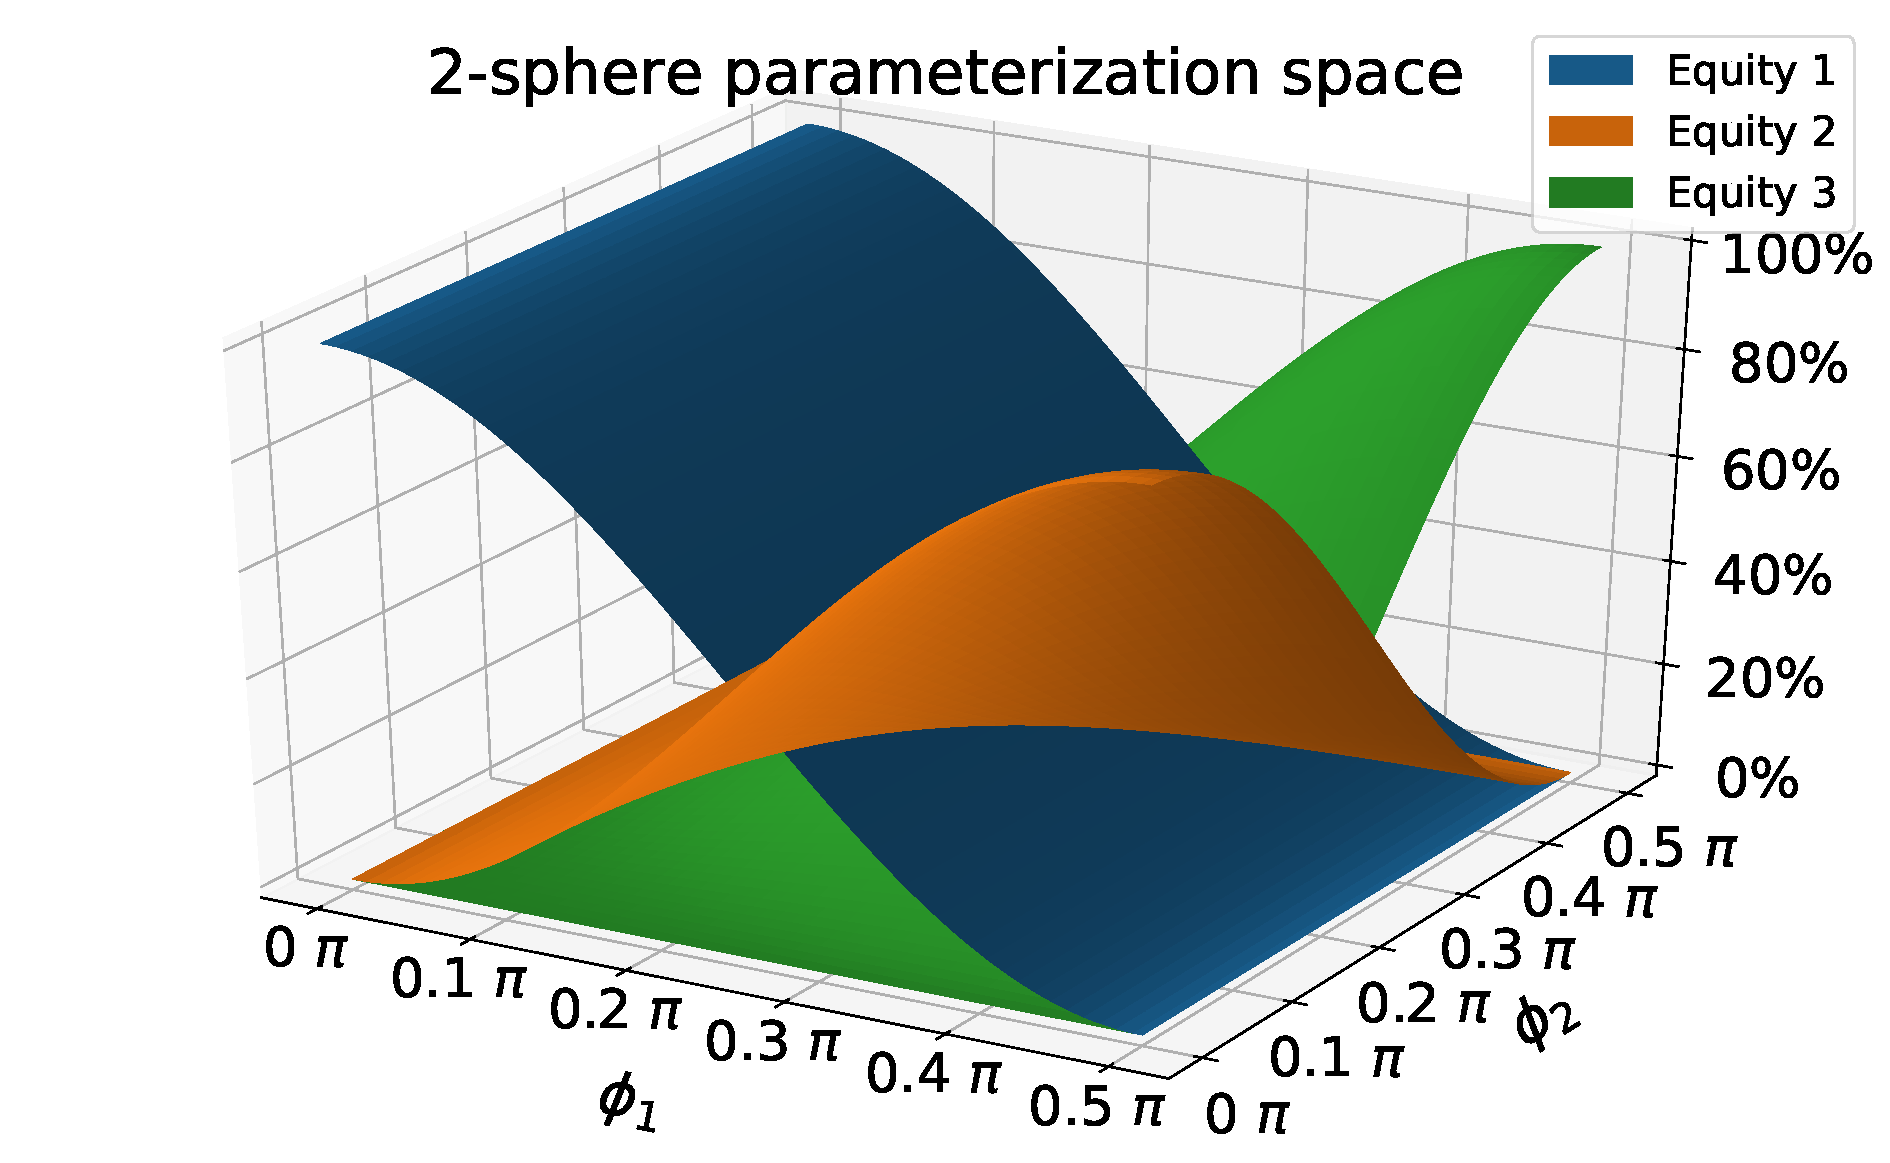
\includegraphics[height=5cm,width=5.8cm]{actionspace3D.pdf}
	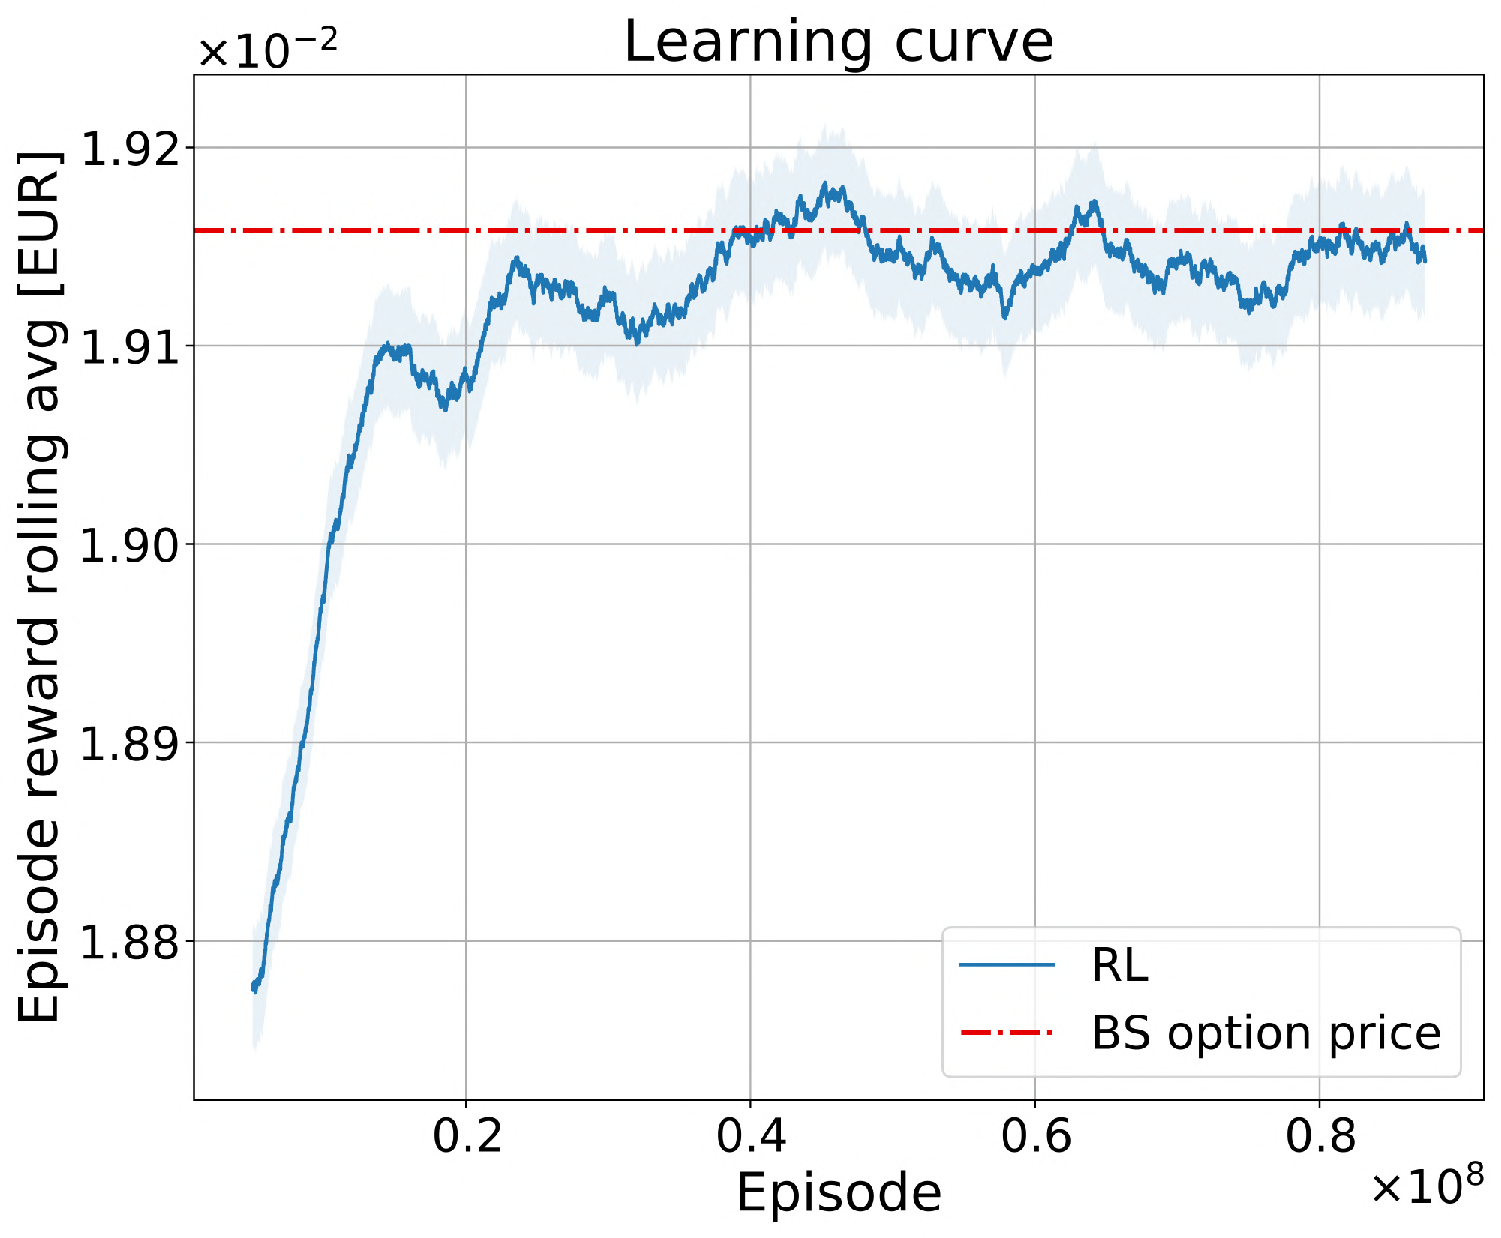
\includegraphics[width=8.3cm,height=6.5cm]{Learning_5x8_marketdata_long_5x8_3asset_beta07_noise05_best_WINDOW5e6_EUR_900dpi}
	
	\caption{On the left $n$-sphere strategy parameterization for 3 equities: $\alpha$ in function of the colatitude $\phi_1$ and latitude $\phi_2$. The domain of the angles is $[0,\pi/2]$. On the right the  learning curve for an agent policy parameterized with $5\times8$ and $\tanh$ as activation function. The agent is trained in a BS environment with three equities. On the horizontal axis the number of training episodes. The solid lines are the moving average of the realized rewards on the last $5\times 10^6$ episodes. The shadows represent the $98\%$ confidence intervals. The dash-dotted horizontal red line is the conservative TVO price computed according to the optimal risky portfolio composition through \cref{eq:bs_closed_solution}.}
	\label{fig:n_sphere_parameterization}
\end{figure}  
\begin{figure}[ht!]
	\centering
	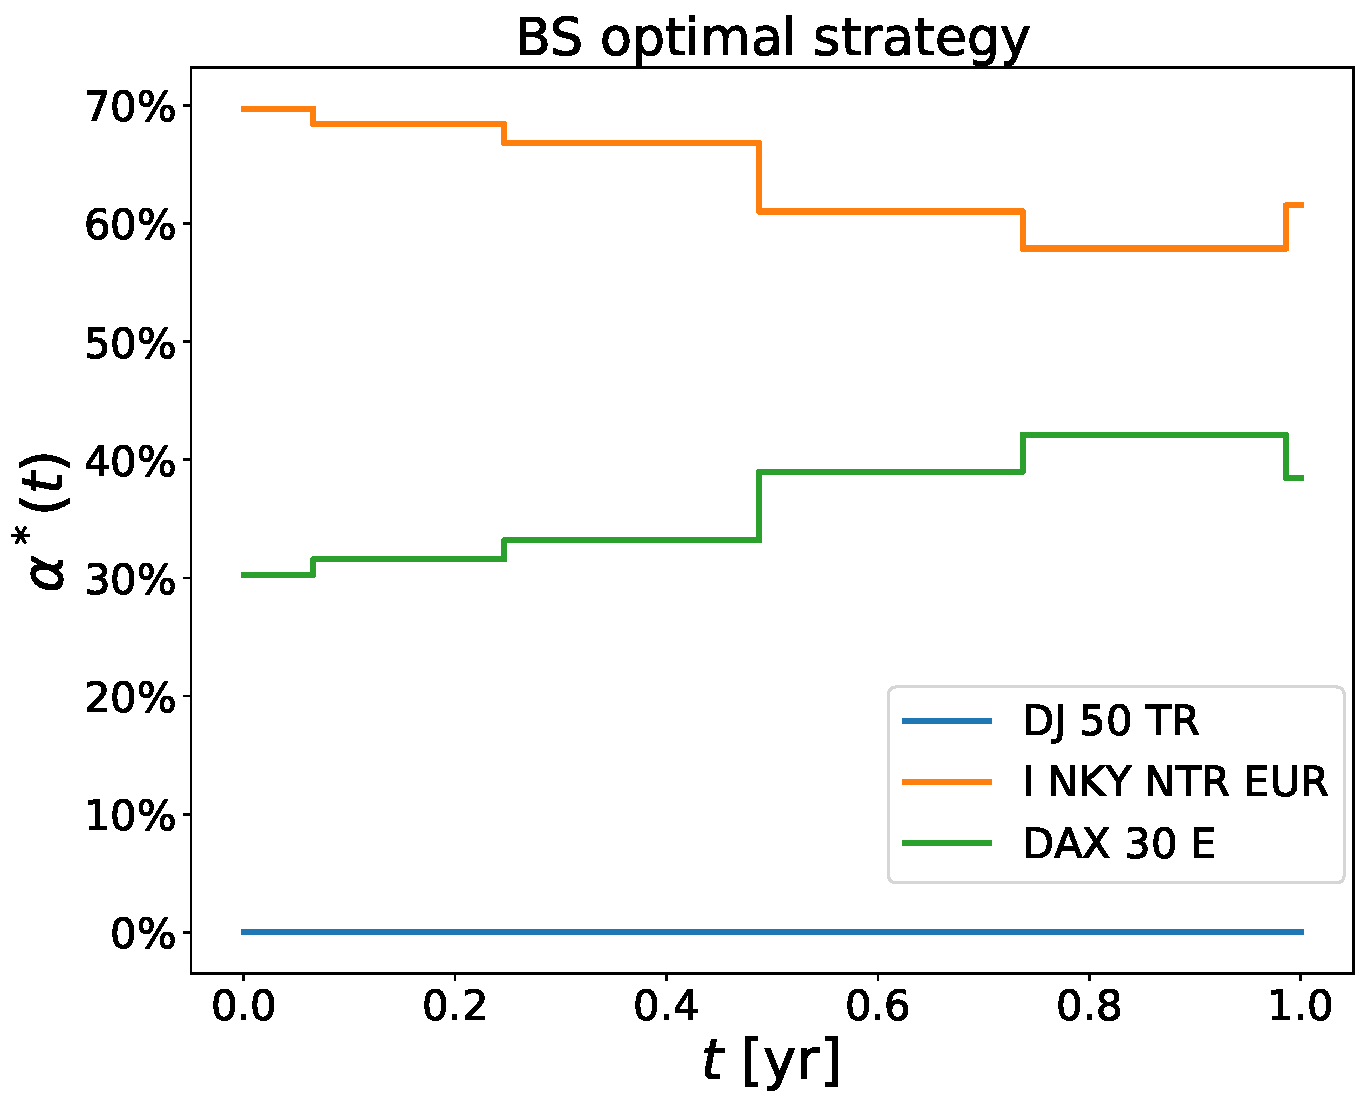
\includegraphics[width=7.2cm,height=6cm]{Instant_Optimal_percentage_strategy_three_assets_real_market.pdf}
	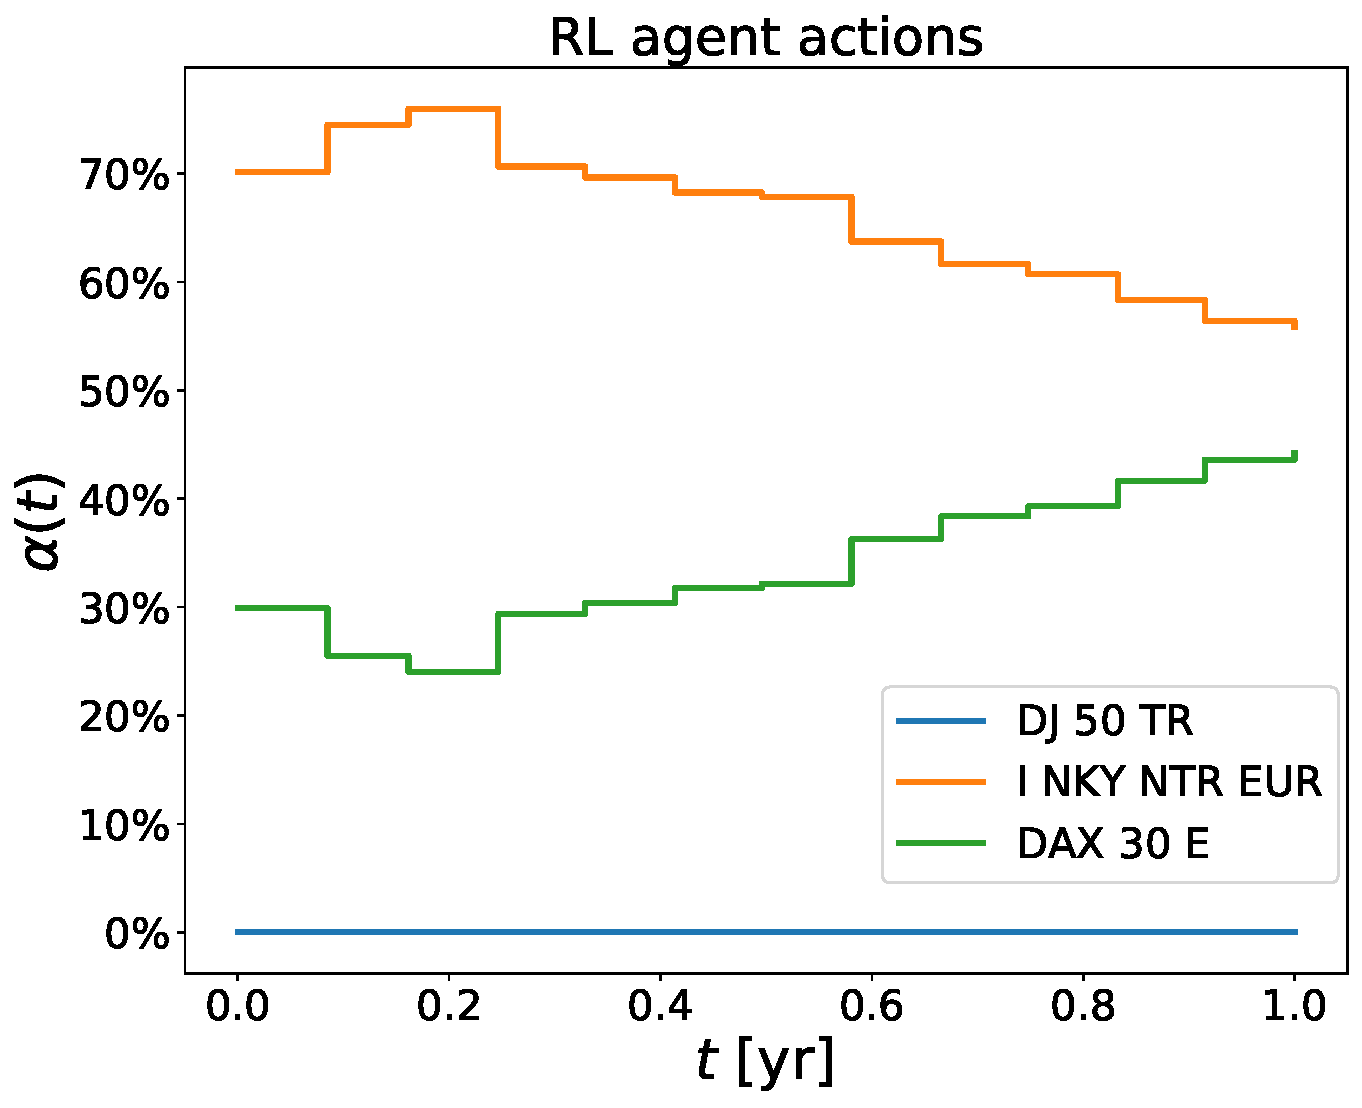
\includegraphics[width=7.2cm,height=6cm]{Action_RL_5x8_marketdata_seed16_long.pdf}
	\caption{Comparison between the BS optimal risky strategy (\Cref{eq:BS_optimal_strategy}) and the RL actions taken in a test episode never seen by the agent. On the horizontal axis time in term of year fractions. The agent training session is showed in \Cref{fig:n_sphere_parameterization}. }\label{fig:RL_actions}\end{figure}

\begin{figure}[ht!]
	\centering
	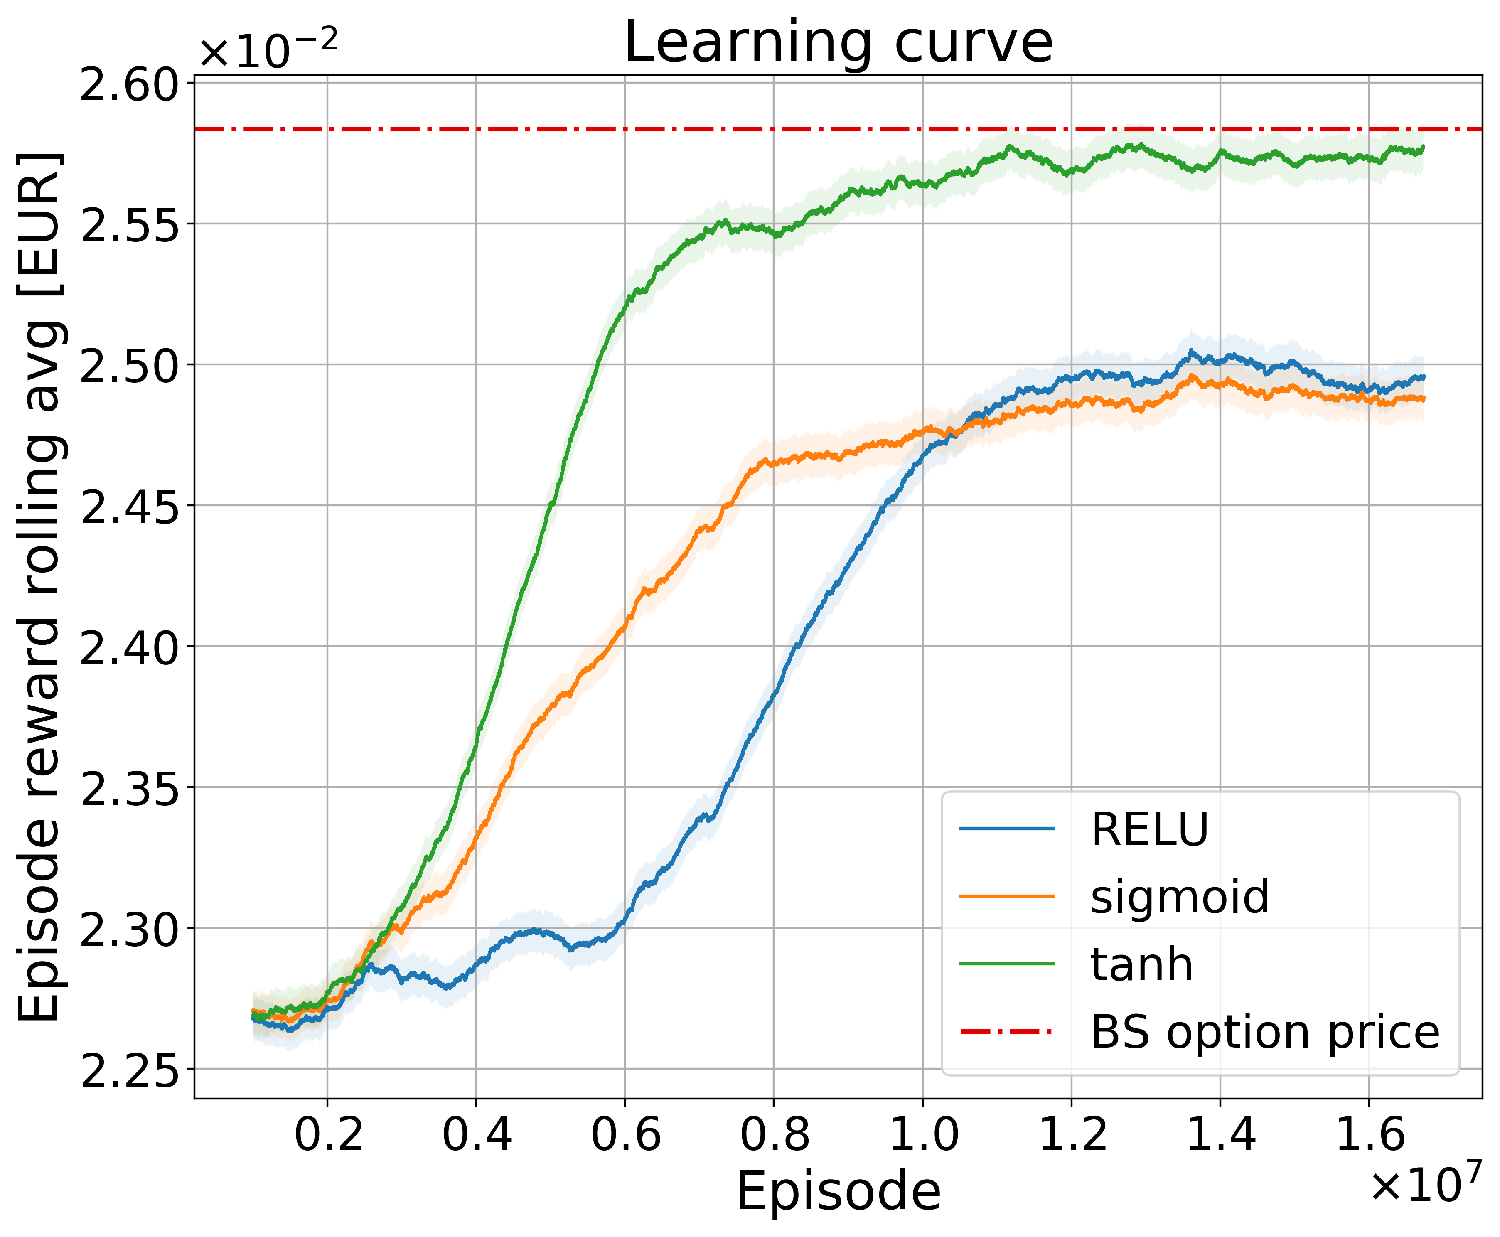
\includegraphics[height=6cm,width=7.2cm]{Activation_functions_Learning_curve_1x40_network_confront_activation_strategy_EUR_8x5_900dpi.pdf}
	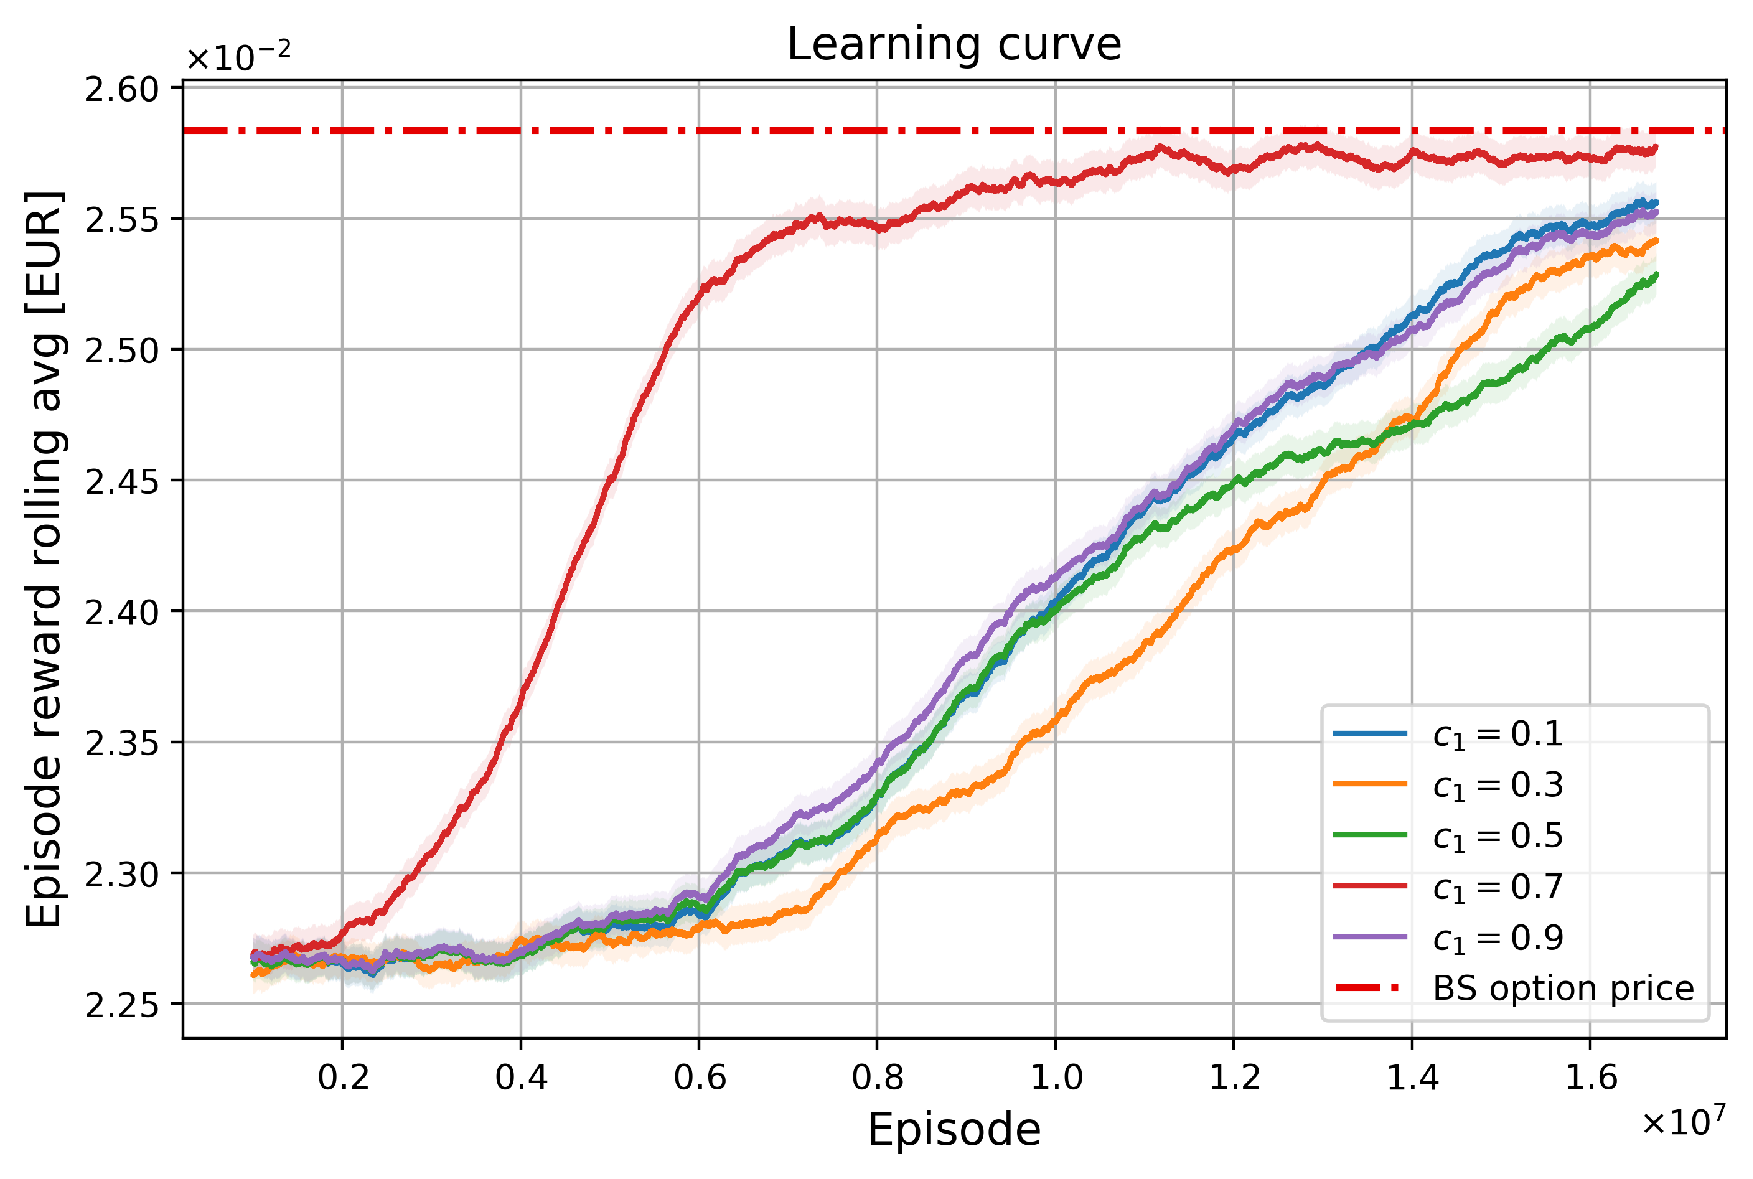
\includegraphics[height=6cm,width=7.2cm]{Value_function_Learning_curve_1x40_beta_confront_varying_strategy_EUR_8x5_400dpi_compressed.pdf}
	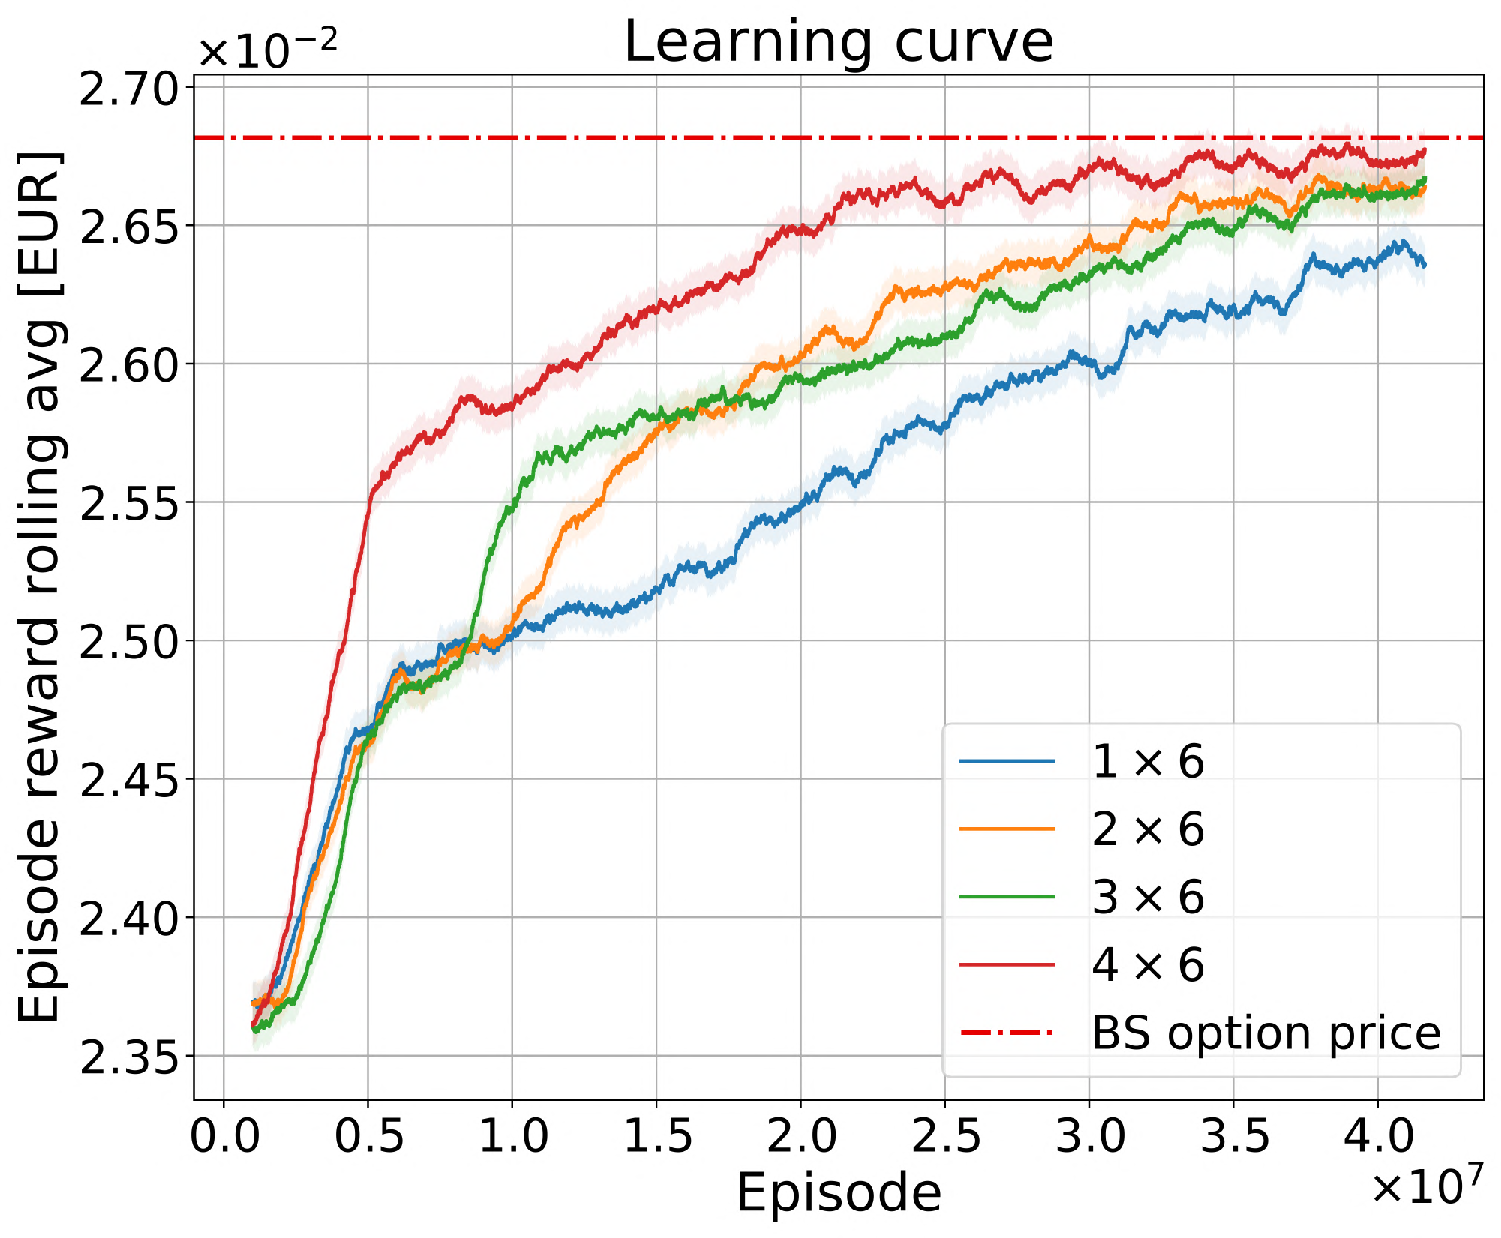
\includegraphics[height=6cm,width=7.2cm]{Hidden_Layers_Learning_curve_3asset_varystrategy_window1000000_EUR_5e8timestep_comparison_900dpi_compressed.pdf}
	\caption{Fine tuning simulations: on the top-left learning curves with different activation functions, on the top-right grid search on the policy-value trade-off and on bottom-centre learning curves on ANNs architectures. On the horizontal axis the number of training episodes. The solid lines are the moving average of the realized rewards on the last $5\times 10^5$ episodes. The shadows represent the $98\%$ confidence intervals. The dash-dotted horizontal red lines are the conservative TVO prices computed according to the optimal risky portfolio composition through \cref{eq:bs_closed_solution}.}
	\label{fig:fine_tuning}
\end{figure}  
\clearpage
\subsection{Local Volatility Dynamics}
In this section we study the TVS control problem assuming a local volatility model for the dynamics of the risky assets. Thus in this case we have a diffusive term in \Cref{eq:Equity_process} that is a deterministic function both of time and state, i.e. the spot price, $\nu_t=\nu(t,S_t)$. This additional dependency of volatility makes the problem of finding the optimal strategy non-trivial; in fact if we consider the whole equity smiles then the second order term in the HBJ equation \eqref{eq:HJB_general} is non null and thus a closed formula for $\alpha^*$ is not available anymore. Because of that one must resort on numerical techniques to recover the problem solution. Unlike BS model where the strategy depends only on time, in LV dynamics there are no unnecessary information provided by the state block in \Cref{eq:state} to take the optimal action. 

We first apply our RL algorithm in the same market data conditions as in the case showed in \Cref{fig:n_sphere_parameterization} on the right, but in the LV dynamics. This choice is done to compare the optimal solution in two well-known financial models. We keep the same ANN architecture as in previous section: a $5\times8$ FFNN with $\tanh$ activation function. This enables us to perform the training using two different initial guesses for the PPO:
\begin{itemize}
	\item \textbf{Random starting point}: the hidden weights $\theta$ of the ANN are randomly initialized so that the training phase starts from a casual policy.
	\item \textbf{Black and Scholes initial guess}: the algorithm initialize the values of $\theta$ with those of the ANN trained in the BS environment. 
\end{itemize}    
The idea behind the second guess is that the LV dynamics differs from BS for a corrective term in the HJB equation and thus we guess that a network which has learnt the BS optimal strategy will be a good starting point for the RL algorithm as sub-optimal value. We present in \Cref{fig:local_vol_learning_curves} on the left the resulting learning curves for two ANNs trained with the two initialization methods just described.   

\begin{figure}[ht!]
	\centering
	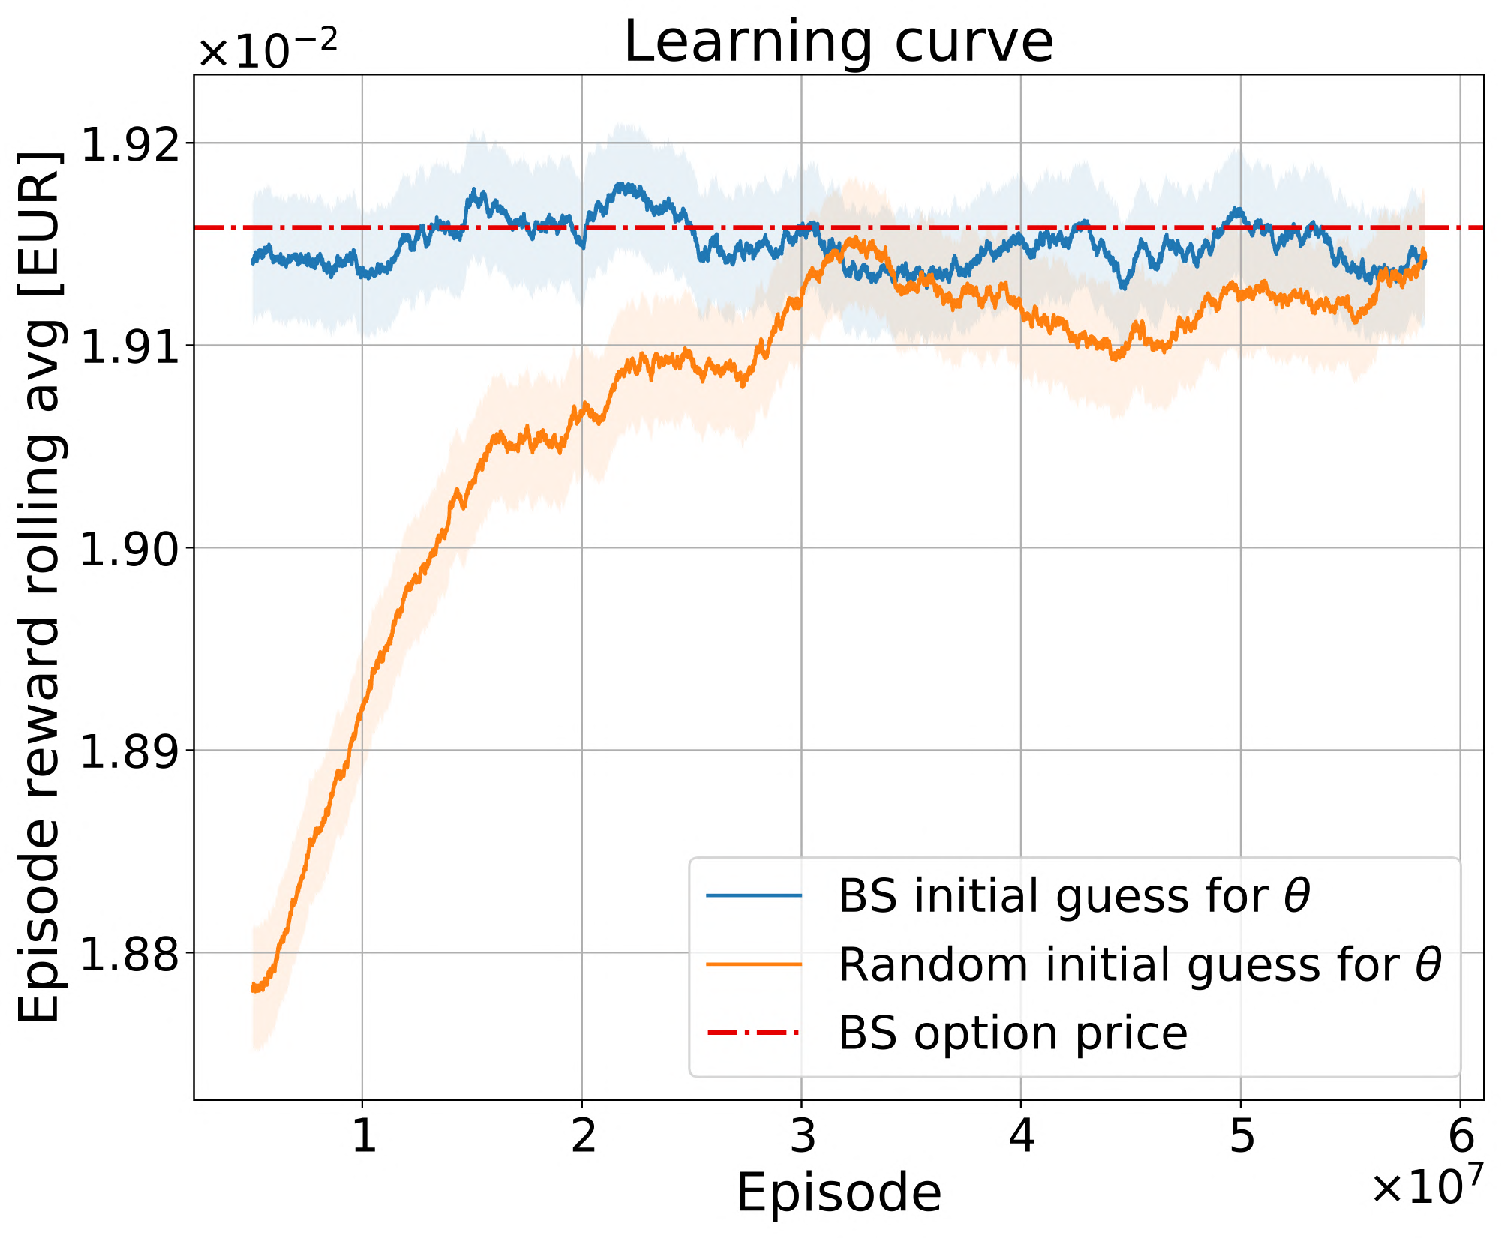
\includegraphics[height=6cm,width=7.2cm]{Learning_curve_all_5x8_localvol_3asset_compressed.pdf}
	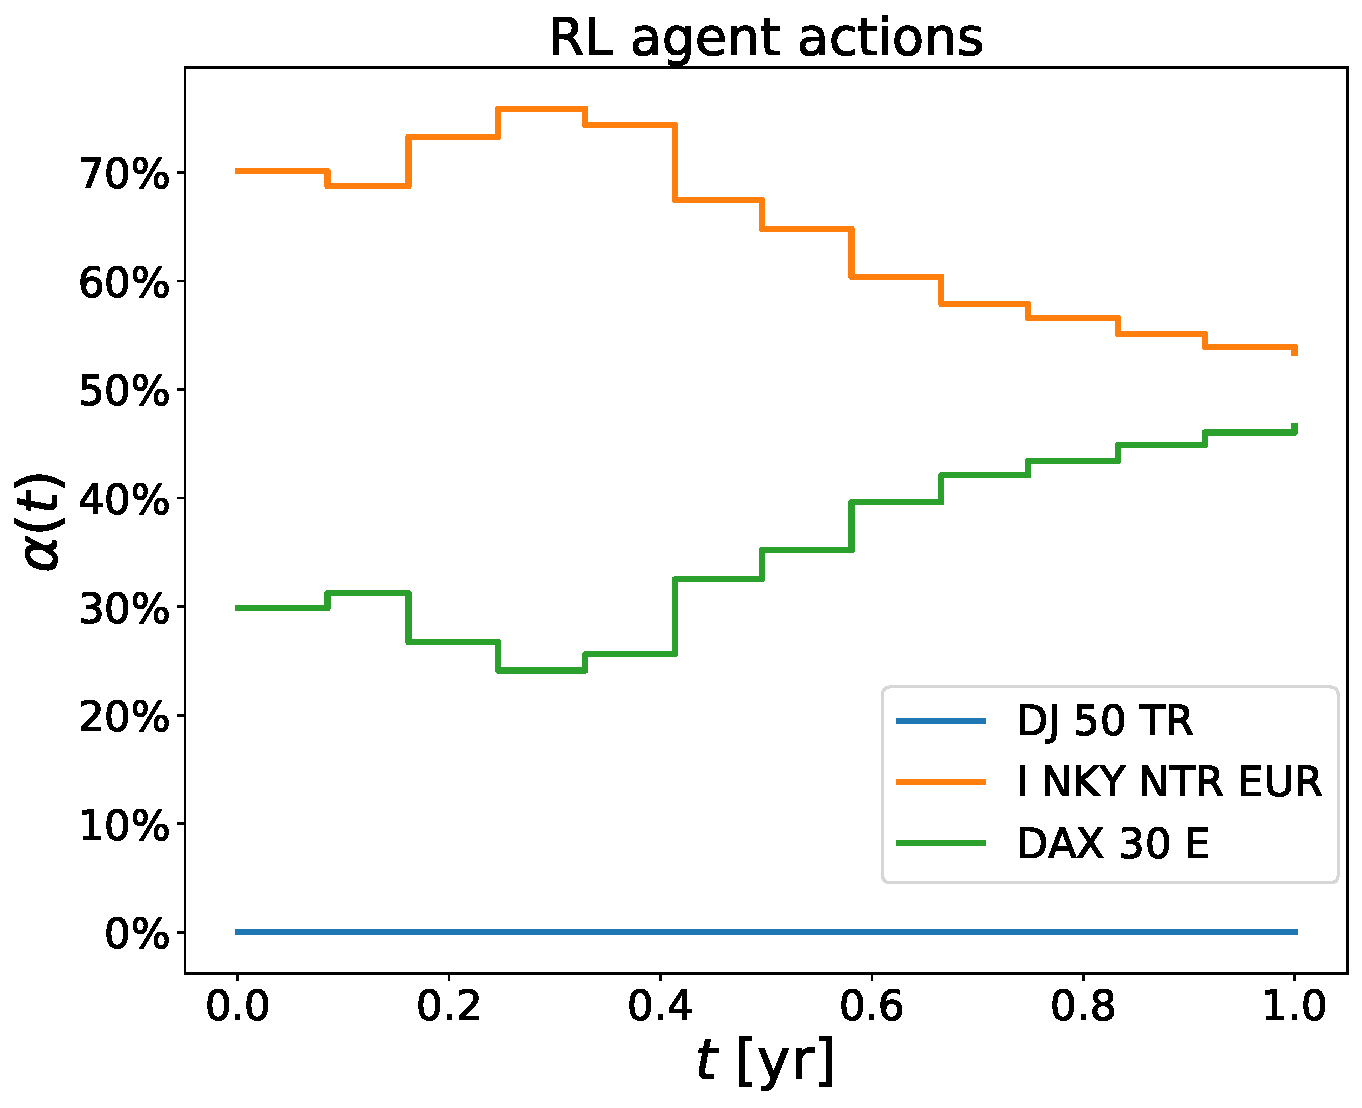
\includegraphics[height=6cm,width=7.2cm]{Action_RL_5x8_marketdata_seed80_long.pdf}
	\caption{On the left, learning curve for two $5\times8$ FFNNs with $\tanh$ activation function and $c_1 = 0.7$.  The networks are both trained in the same LV but with different starting point: random policy for the orange line and BS optimal policy for the blue one. The dash-dotted horizontal red line is the conservative BS call option price  computed according to the optimal risky portfolio in \Cref{fig:RL_actions} on the left.
	On the right agent actions in a never-seen MC episode.	
}
	\label{fig:local_vol_learning_curves}
\end{figure}  

\noindent Analyzing the training results, we observe that the two curves converges both to the same saturation value which is compatible with the optimal BS price for the TVO curve. The RL agent has learnt in both cases the optimal allocation strategy of the BS model. In fact if we plot the agent actions taken in never-seen scenarios (\Cref{fig:local_vol_learning_curves} on the right), we see that they are in accordance with those of BS. 

As told before, in the LV model the optimal strategy is not available \textit{a priori} as in BS and thus we can not say if the solution found by the RL agent is sub-optimal. However we can check if the agent is stuck in a local optimum by building a n\"aif strategy to measure the performance of the RL algorithm; we call this strategy \virgolette{baseline}. Since we have proved in \Cref{subsec:BS_model} that in the BS model the solution is the allocation strategy that maximizes the local drift of the TVS, we choose as baseline a manager that applies path-wise the BS solution \eqref{eq:BS_optimal_strategy}. 
In \Cref{tab:mc_results_lv} we compare the MC prices obtained applying in $10^6$ paths the baseline and the ANNs trained before.
\begin{table}[t]
	\centering
	\begin{tabular}{|c|c|} \hline
		Method & TVO price [EUR]  \\ \hline 
		RL from random $\theta$ & $(1.912 \pm 0.003) \times 10^{-2}$ \\
		RL from BS $\theta$ & $(1.915 \pm 0.003) \times 10^{-2}$ \\
		Baseline & $(1.915 \pm 0.004) \times 10^{-2}$ \\ \hline
	\end{tabular}\caption{MC prices of an atm-spot TVO with LV dynamics for the risky assets and with $K=1\,[\text{EUR}]$, $T = 1\,[\text{yr}]$ and $\bar{\sigma}=5\%$.  The prices are obtained computing three different allocation strategies: the ANN trained starting from a random policy, the ANN trained from the BS strategy and the baseline. }
	\label{tab:mc_results_lv}\end{table}
All the prices computed with different strategies are $2\sigma$-compatible among them. Thus we can assert that in the market data conditions we have considered, the LV optimal strategy coincides with the BS one. Moreover we observe that the baseline strategy and the BS optimal one provide the same TVO price, such as the risky securities dynamics is irrelevant for the resulting price. 

Thus we try different configurations for the hedging costs $\mu_t$ and the implied volatility (IV) surfaces in order to find a market where the TVO prices reached by the baseline and by the BS optimal strategy differ between them. From our analyzes we have evidence that in markets where the risky equities have different hedging costs, then the baseline and the BS solution gives the same TVO prices and optimal strategies; this is due to the fact that the numerator in \Cref{eq:BS_optimal_strategy} plays an important role in the minimization and thus in the problem solution. For this reason we consider a market of two equities with two different shapes for the smiles curves and a $\mu_t$ vector that has equal positive entries. In particular we choose a symmetric smile for one equity and a displaced diffusion for the second one (\Cref{fig:displaced_diffusion} on the left). In this way the BS optimal solution with long constraint depends only on the diffusive term:
\begin{equation}
	\alpha^*(t) = \mu(t)\argmin_\alpha \|\alpha\cdot\nu(t)\|^{-1}.
\label{eq:BS_strategy_particular_equal_repo}\end{equation}    
In a similar way the baseline
\begin{equation}
	\alpha^*(t,S_t) = \mu(t)\argmin_\alpha \|\alpha\cdot\nu(t,S_t)\|^{-1}.
\label{eq:baseline_strategy}\end{equation}
Therefore, having a completely different smiles curves will make differ the BS solution from the baseline one since the former is computed with a diffusive term $\nu(t)$ obtained by interpolating linearly the IV curve on the atm-spot strike and thus loosing all the information about the $K$-dependence. We train the RL agent in this market configuration by parameterizing the actions with the baseline strategy. In particular at each observational time $T_K\in\mathcal{T}$ the risky allocation strategy is obtained by summing the ANN output with the \eqref{eq:baseline_strategy} and then remapped so that the long only strategy constraint is satisfied. We adopt this parameterization to help the agent find the optimal strategy as correction to the baseline one. We report in \Cref{fig:displaced_diffusion} on the right the resulting learning curve compared with the TVO price adopting the state-independent BS strategy \eqref{eq:BS_strategy_particular_equal_repo} and with the baseline \eqref{eq:baseline_strategy}. We observe that it learns as optimal policy the baseline strategy. We obtain the same result by adopting the second reward function \eqref{eq:reward} and decreasing the $\gamma$ discount factor to make the agent prefer immediate rewards. 
\begin{figure}[ht!]
	\centering
	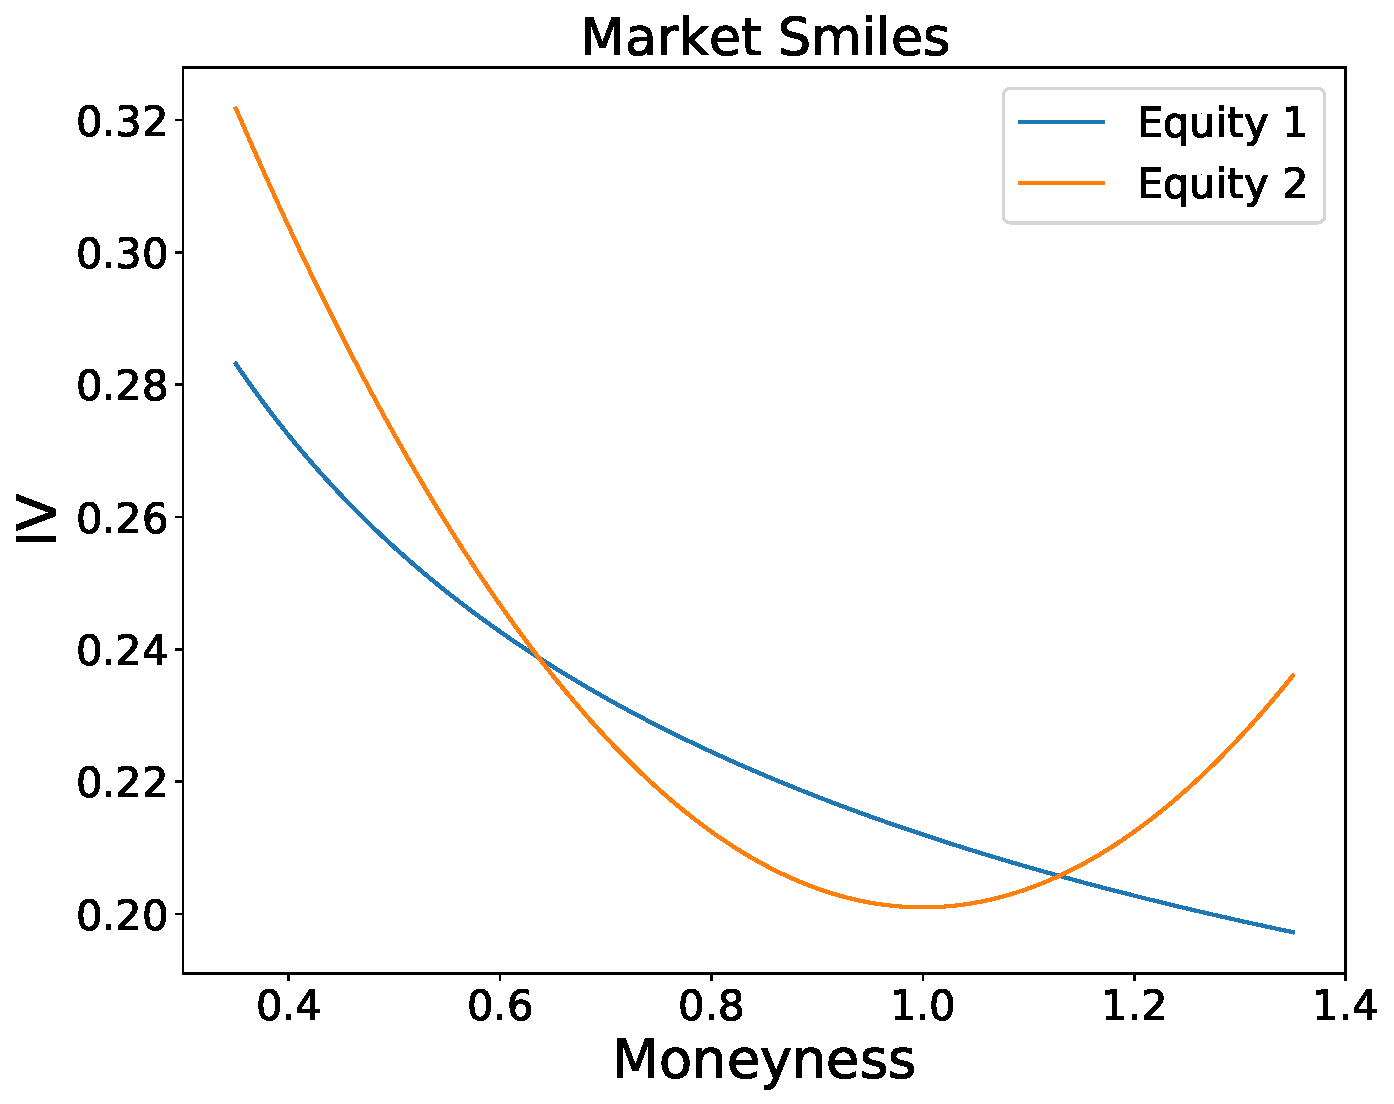
\includegraphics[height=6cm,width=7.2cm]{SmileDisplacedDiff.pdf}
	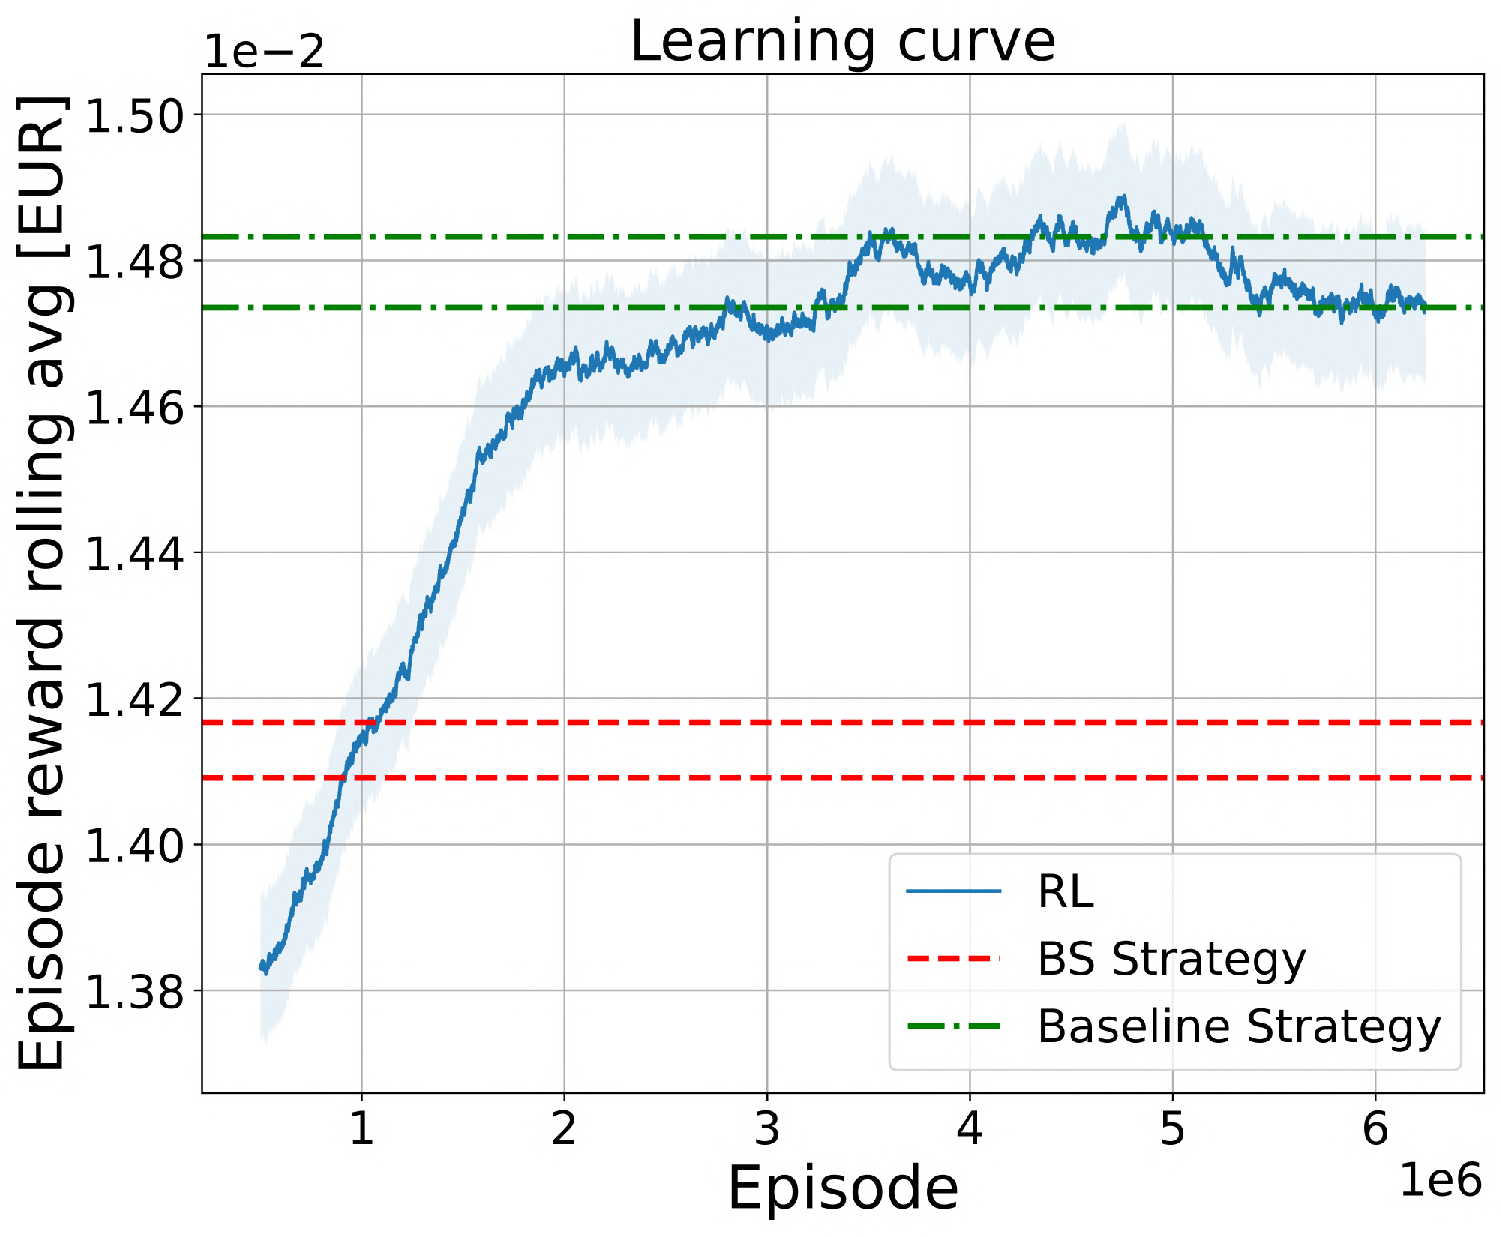
\includegraphics[height=6cm,width=7.2cm]{Learning_curve_market_displaced_compressed.pdf}
	\caption{On the left market smiles for two equities in function of moneyness: symmetric smile at atm for equity 2 and displaced diffusion for equity 1. On the right learning curve for a $5\times8$ ANN trained in the LV market with the smile curves on the left. The learning curve is compared with the baseline and the static BS strategies. }
	\label{fig:displaced_diffusion}
\end{figure} 


\section{Conclusion and Further Developments}
In this paper we described a non-trivial control problem related to derivative contracts on target volatility strategies. We considered a bank selling a call option to a fund manager as protection  on the capital
invested on the TVS. We showed how the presence of different funding costs coming from hedging the risky assets underlying the TVS, makes the bank solving a stochastic optimal control problem to adjust the price of the protection, since the bank strategy is not self-financing. We derived a closed form solution of the control problem in a Black and Scholes framework in two different ways: first by applying the Gy\"ongy  Lemma and then by writing the Hamilton-Jacobi-Bellman equation. We studied the problem both in the BS world and in the local volatility one where the solution is not available and thus numerical investigation is needed. We tackled the problem by means of the novel Reinforcement Learning techniques, such as the proximal policy optimization. We used the BS model, where the solution is \textit{a priori} known, as benchmark to perform a series of fine-tuning of the RL algorithm hyper-parameters, such as the artificial neural network architecture. Then we investigated the problem under LV dynamics. From our simulations we had evidence that under this model the RL agent learnt as optimal strategy the application path-wise of the BS solution. This topic is still under study since our results for the LV model do not provide a formal demonstration of that the problem solution is the path-wise BS one. For this reason the natural developments of this work is to compare our RL results with other standard techniques like the least-square Monte Carlo. If the resulting comparison is positive, then it will provide robustness of our LV results.
\begin{comment}


In the Black and Scholes environment we study some markets composed by simple 
\begin{figure}[ht!]
\centering
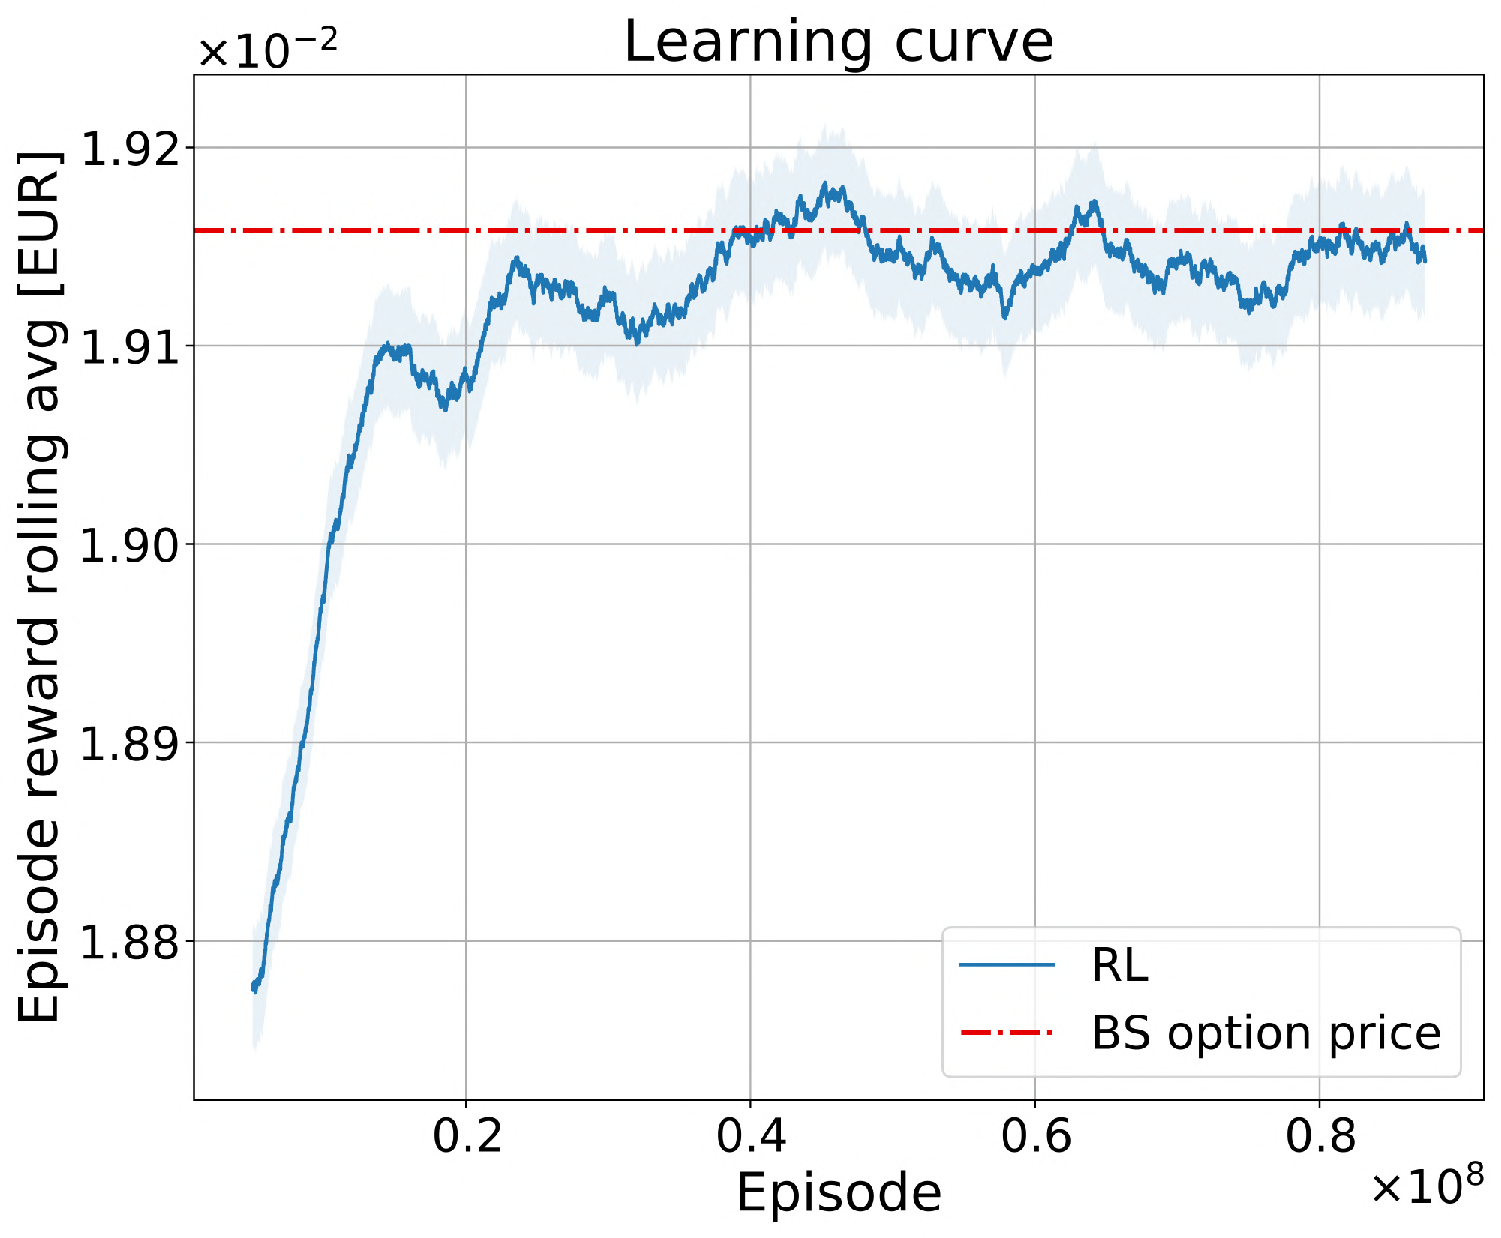
\includegraphics[width=10cm,height=7cm]{Learning_5x8_marketdata_long_5x8_3asset_beta07_noise05_best_WINDOW5e6_EUR_900dpi}
\caption{Learning curve for an agent policy parameterized with $5$ layers, $8$ neurons per layer and $\tanh$ as activation function. The agent is trained in a BS environment with three equities. On the horizontal axis the number of training episodes. The solid lines are the moving average of the realized rewards on the last $5\times 10^6$ episodes. The shadows represent the $98\%$ confidence intervals. The dash-dotted horizontal red line is the conservative TVO price computed according to the optimal risky portfolio composition through \eqref{eq:bs_closed_solution}.}
\label{fig:Learning_curve_3asset_BS}\end{figure}

 In the last section we provide a first analysis of the LV model where a closed strategy is not available. The BS environment is used as a toy model in order to understand which parametersof the ANN and of the PPO play key roles in our RL algorithm. 

\subsection{Black and Scholes Dynamics}
--normalizzazione degli input.
\subsection{Local Volatility Dynamics}
\section{Discussion}
\end{comment}
\begin{comment}

--scrivere input normalization della rete
--introduzione sui modelli fatti 
--dire perch� black e del fine tuning dei parametri 


%%Buona simulazione local vol [ ppo2_1.5e8_5x8_3e-4frombaselinelong_displacedmarket_month_2assets_beta0.7_maturity2_seed5343061 ] su macchina remota in TVS_LV-v0


\ref{sec:target_volatility_option_derivative_pricing}, the bank evaluation of the most conservative call option price strictly depends on the dynamics followed by the equities underlying the \acrshort{tvs}; in particular the volatility term of the securities affects the \acrshort{tvs} price process \eqref{TVS_last}. In our work we will try to solve this pricing problem through the \acrshort{rl} technique, training the agent in two different environments corresponding to two different mathematical models for the dynamics of financial markets: the time-dependent \acrlong{bs} model and the \acrlong{lv} model. Although the first one is quite simple (its parameters depends only on time) and it is not completely able to represent the complex dynamics of real markets, we have seen that, under Black's conditions, we are able to derive the closed form solution for the optimal strategy \eqref{optimal_strategy}. Thus we can use the \acrlong{bs} model as a test to control if we have built correctly the \acrlong{rl} algorithm; in other words we will check if the \acrshort{rl} agent will take decisions in agreement with the closed form. On the other hand, the \acrfull{lv} model depends not only on time but also on the spot prices of the equities and thus a closed formula for the optimal strategy is not available; we will try to recover it by our \acrshort{rl} algorithm.


The actions of the agent as a function of its observations of the environment are termed the agent policy.  In our case the policy is the asset allocation weights $\alpha$, while the rewards are the costs generated by hedging a derivative contract on the TVS. Once the agent is trained, and the optimal policy is selected, we can run a Monte Carlo simulation to calculate the option price on the TVS. 
 
 We adopt as learning strategy the PPO algoritm developed in \textcite{ppo} and \textcite{gae}. We have 
\end{comment}
\\

\printbibliography
\end{document}
